% options:
% thesis=B bachelor's thesis
% thesis=M master's thesis
% czech thesis in Czech language
% slovak thesis in Slovak language
% english thesis in English language
% hidelinks remove colour boxes around hyperlinks

\documentclass[thesis=M,czech]{FITthesis}[2012/06/26]

\usepackage[utf8]{inputenc} % LaTeX source encoded as UTF-8
\usepackage{float}
% \usepackage{amsmath} %advanced maths
% \usepackage{amssymb} %additional math symbols
\usepackage{subfig,graphicx}
\usepackage{array}
\usepackage{color}
\usepackage{makecell}

\usepackage{dirtree} %directory tree visualisation
\usepackage{lscape}
\usepackage{hyperref} %todo přidat do normální hlavičky %
\usepackage{longtable}

% % list of acronyms
% \usepackage[acronym,nonumberlist,toc,numberedsection=autolabel]{glossaries}
% \iflanguage{czech}{\renewcommand*{\acronymname}{Seznam pou{\v z}it{\' y}ch zkratek}}{}
% \makeglossaries

\newcommand{\tg}{\mathop{\mathrm{tg}}} %cesky tangens
\newcommand{\cotg}{\mathop{\mathrm{cotg}}} %cesky cotangens
\newcommand{\ptheory}{$\Psi$-theory}

% % % % % % % % % % % % % % % % % % % % % % % % % % % % % % 
% ODTUD DAL VSE ZMENTE
% % % % % % % % % % % % % % % % % % % % % % % % % % % % % % 

\department{Katedra softwarového inženýrství}
\title{Možnosti využití metodiky DEMO pro tvorbu BPMN modelů}
\authorGN{Štěpán} %(křestní) jméno (jména) autora
\authorFN{Heller} %příjmení autora
\authorWithDegrees{Bc. Štěpán Heller} %jméno autora včetně současných akademických titulů
\supervisor{Ing. Pavel Náplava}
\acknowledgements{Rád bych poděkoval mému vedoucímu Ing. Pavlu Náplavovi za cenné rady v průběhu tvorby práce a také Stevenu Van Kervelovi ze společnosti Formetis, jehož postřeby byly velkým přínosem pro vznik této práce.}
\abstractCS{Tato diplomová práce se zabývá kombinací silných stránek notace BPMN (Business Process Model and Notation) a metodologie DEMO (Design \& Engineering Methodology for Organizations). Za silné stránky notace BPMN v tomto kontextu autor označuje zejména srozumitelnost pro business uživatele a dále širokou paletu nástrojů, které umožňují modelování podnikových procesů v BPMN. V případě metodologie DEMO autor identifikuje silné stránky v hlubokém teoretickém základu, který zajišťuje vytváření modelů, které jsou ontologicky kompletní, konzistentní a jsou oproštěné od implementačních detailů.

V této práci čtenář nalezne srovnání běžných technik pro modelování podnikových procesů a dále hlubokou analýzu BPMN a DEMO. Hlavním přínosem této diplomové práce je však předpis, jak mapovat základní koncepty metodologie DEMO na BPMN primitiva a především návrh metody, jak využít důležité teoretické koncepty metodologie DEMO pro tvorbu BPMN modelů, které jsou kompletní, konzistentní, jednoznačné a esenciální. Navržená metoda je dále demonstrována na příkladu.}
\abstractEN{This thesis combines the strong aspects of BPMN (Business Process Model and Notation) such as good understanding of the notation among business users and large amount of software tools available that support the notation with strong aspects of DEMO (Design \& Engineering Methodology for Organizations) such as the profound theoretical background which assures the user that the model he gets as a result is ontologically complete, consistent and abstracts away from all unnecessary implementation details.

This thesis contains an analysis of available business process modelling techniques along with a thorough analysis of BPMN and DEMO. The main contribution of the thesis however is a proposal of a method that makes use of important theoretical concepts of DEMO in order to create BPMN models which are complete, consistent, unique and essential. The use of the method is then demonstrated on an example.}
\placeForDeclarationOfAuthenticity{V~Praze}
\declarationOfAuthenticityOption{4} %volba Prohlášení (číslo 1-6)
\keywordsCS{DEMO, Design \& Engineering Methodology for Organizations, BPMN, Business Process Model and Notation, Enterprise ontology, Business Process Management, Proces, Procesní model}
\keywordsEN{DEMO, Design \& Engineering Methodology for Organizations, BPMN, Business Process Model and Notation, Enterprise ontology, Business Process Management, Process, Process Model}

\begin{document}

% \newacronym{CVUT}{{\v C}VUT}{{\v C}esk{\' e} vysok{\' e} u{\v c}en{\' i} technick{\' e} v Praze}
% \newacronym{FIT}{FIT}{Fakulta informa{\v c}n{\' i}ch technologi{\' i}}

\begin{introduction}
	Každá organizace (nezáleží zda firma, úřad nebo spolek) od určité velikosti začne řešit problémy s efektivitou a udržitelností růstu. Jedním z řešení, ať už k němu řídící pracovníci přistoupí vědomě či nevědomě, je nějaká forma \textit{procesního řízení}.

Procesní řízení, jehož základům se podrobně věnuje kapitola 1, ve své podstatě znamená standardizaci opakujících se postupů, jejich zaznamenání ve formě, která umožní pozdější analýzu a optimalizaci za účelem zvyšování efektivity jejich provádění a eliminaci chyb, které mohou vzniknout.

Přístupy, jak procesy zaznamenávat, analyzovat a optimalizovat se vyvíjí stejně jako se vyvíjí organizace, společnost, požadavky zákazníků a v neposlední řadě technologie. Od intuitivního zaznamenávání průběhu procesů pomocí \textit{vývojových diagramů}, které neumožňovaly nic jiného než prosté grafické znázornění posloupnosti aktivit, se vývoj posunul k automatizaci procesů pomocí výpočetních prostředků a analýze velkého množství dat o každém kroku analyzovaného procesu.

Tato práce se snaží přispět k tomu, aby bylo možné procesy zaznamenávat a analyzovat s větší mírou konzistence podle metody, jejíž návrh tato práce představuje v kapitole 5.

\subsection{Motivace}
V této práci jsou analyzovány dvě techniky použitelné k modelování podnikových procesů – DEMO a BPMN. BPMN je v současnosti zřejmě nejpoužívanější notací pro vizuální reprezentaci podnikových procesů. Její předností je zejména velká srozumitelnost pro business uživatele, kteří jsou dobře obeznámeni s vývojovými diagramy a jsou tak schopni číst i vytvářet diagramy v BPMN bez větších problémů. Slabinou BPMN je však absence jasných pravidel \textit{jak} diagramy vytvářet, \textit{které} části procesu v nich zaznamenávat a \textit{z čeho} se procesy vlastně skládají. Výsledkem jsou BPMN modely, které jsou často \textit{nekompletní}, \textit{nekonzistentní} a \textit{nejednoznačné}.

DEMO je metodologie založená na silném teoretickém základu, který se skládá především z \textit{Enterprise ontology} a \textit{\ptheory}. DEMO má jasná pravidla co v modelech zachycovat, jak při vytváření modelů postupovat a jak ověřit, zda jsou vzniklé modely korektní a správné. Metodologie DEMO zajišťuje, že pokud dodržíme veškeré postupy, které tato metodologie stanoví, tak nám při modelování stejného procesu musí na konci vždy vzniknout ten samý model. Tato jistota má zásadní pozitivní důsledky pro analýzu, sdílení i diskusi nad procesy v rámci organizace.

Tato práce si klade za cíl zkombinovat výhody obou technik, tedy dobrou srozumitelnost business uživateli na straně jedné a pevný teoretický základ na straně druhé, vyvinutím metody, která umožní vytvářet BPMN modely, které budou \textit{kompletní}, \textit{konzistentní} a \textit{jednoznačné}. V kombinaci s možnostmi automatizace by se mohlo jednat o krok dopředu v celé oblasti Business Process Managementu.

\subsection{Struktura práce}
Práce je rozdělena do šesti kapitol. V první jsou definovány základní pojmy, se kterými je ve zbytku textu pracováno a také je zde rozebrán vývoj přístupů k práci s podnikovými procesy. Druhá kapitola analyzuje nejpoužívanější techniky pro modelování podnikových procesů a srovnává jejich silné a slabé stránky. Třetí a čtvrtá kapitola rozebírají notaci BPMN, respektive metodologii DEMO do hloubky – jejich základní principy a postupy. V páté kapitole se nachází klíčová část této práce, kterou je jednak jednak návrh toho, jak vyjádřit klíčové prvky metodologie DEMO pomocí primitiv z notace BPMN a také návrh metody, která obsahuje sedm kroků dle kterých je možné vytvořit BPMN model procesu. Výsledný model by měl být \textit{kompletní}, \textit{konzistentní} a \textit{jednoznačný}. Závěrečná kapitola demonstruje navrženou metodu na konkrétním příkladu a diskutuje výsledky její aplikace.

\subsection{Překlad cizojazyčných termínů}
Při psaní textu se autor potýkal s problémem, že zejména v případě metodologie DEMO existuje jen mizivé množství textů v českém jazyce, které by popisovaly tuto metodologii. Základní termíny, kterými jsou označeny jednotlivé prvky metodologie, tak nemají český překlad. Autor se rozhodl toto řešit částečným překladem těch termínů, u kterých je přeložení přímočaré a jinak pracoval s původními anglickými výrazy. Při případné aktualizaci práce by bylo možné přeložit více termínů, pokud by se na českých ekvivalentech našla shoda v rámci české komunity DEMO.

\subsection{Klíčové zdroje}
Pro čerpání informací použil autor této diplomové práce několik desítek zdrojů, ale tři níže uvedené stojí za vypíchnutí a krátký komentář, neboť byly pro vznik této práce zásadní.

\subsubsection{Enterprise ontology – Jan L. G. Dietz}
Jan Dietz je tvůrcem metodologie DEMO a autorem celé řady publikací na téma fungování organizací, sociálních interakcích v nich, stejně jako na modelování jejich činnosti. Kniha \textit{Enterprise ontology – Theory and Metodology} podrobně popisuje všechny tyto fenomény stejně jako Enterprise ontology, \ptheory a celou metodologii DEMO.

\subsubsection{Enhancing the Formal Foundations of BPMN by Enterprise Ontology – Van Nuffel, Mulder, Van Kervel}
Tato publikace je jednou z mála, které se zabývají nějakým druhem kombinace DEMO a BPMN. V tomto případě se jedná zejména o analýzu již existujících BPMN modelů z hlediska požadavků na ontologickou kompletnost a konzistentnost. Tato práce zároveň obsahuje postup, jak zajistit úpravu těchto BPMN modelů tak, aby tyto požadavky splňovaly.

V této souvislosti by autor rád zmínil, že v rámci tvorby této diplomové práce navštívil jednoho z autorů této publikace Stevena Van Kervela a jeho tým ve společnosti Formetis, za účelem diskutování závěrů a přínosů práce. Tato návštěva byla pro vznik této diplomové práce velkým přínosem.

\subsubsection{Business Process Modeling and Simulation: DEMO, BORM and BPMN – Zuzana Vejražková}
Třetí publikací, která byla zásadní pro vznik této diplomové práce je diplomová práce Zuzany Vejražkové, která vznikla na Fakultě informačních technologií ČVUT. Tato práce se zabývá analýzou technik DEMO, BORM a BPMN s důrazem na simulaci podnikových procesů, která umožňuje jejich efektivnější analýzu.

Rozdíl mezi touto diplomovou prací a prací Zuzany Vejražkové je jednak ve volbě technik, které jsou zkombinovány (Zuzana Vejražková kombinuje DEMO s Petriho sítěmi, tato práce kombinuje DEMO a BPMN) a jednak v menším důrazu na simulaci a automatizaci, kterou autor této diplomové práce přenechává dalšímu výzkumu.
\end{introduction}

\chapter{Definice základních pojmů} \label{chap:1}
	\documentclass[]{article}
\usepackage[czech]{babel}
\usepackage[utf8]{inputenc}

\begin{document}

\title{Kapitola 1: Definice základních pojmů}
\author{Bc. Štěpán Heller}
\date{\today}
\maketitle

\section{Motivace k řízení podnikových procesů}
Každá firma, která se snaží efektivně řídit svůj chod a neustále se rozvíjet stále hledá nové a nové cesty, jak toho docílit. Takovými cestami může být uvádění nových produktů na trh, hledání nových trhů a příležitostí na nich, nabírání nových zaměstnanců, investice do propracovaného marketingu a mnoho dalších. Stále více firem ale v posledních několika dekádách obrací svou pozornost také dovnitř vlastní organizace. Hledají oblasti, kde je možné najít úspory nebo kde by bylo možné práci zefektivnit.

Aby bylo něco takového vůbec možné, musí mít manažeři a odpovědní vedoucí pracovníci především přehled o své organizaci a její hlubokou znalost. Pouze z takové hluboké znalosti pak mohou vzejít příležitosti k efektivnějšímu dosahování podnikových cílů.

Z toho důvodu firmy a organizace hledají cesty, jak lépe pochopit a následně standardizovat \textit{procesy} v rámci vlastního podniku, které ve svém souhrnu nejsou nic jiného než soubor postupů, kterými podnik nebo organizace dosahuje svých cílů. O tom, kterak takové procesy pozorovat, standardizovat a řídit, byla napsána celá řada publikací a je nezbytné mít na zřeteli, že se jednotlivé přístupy od sebe více či méně odlišují. 

Ačkoliv akademici i odpovědní lidé z prostředí samotných firem a organizací se často přou, který z přístupů je lepší, zůstává bez nejmenších pochyb, že adoptování jakéhokoliv přístupu vedoucího k lepšímu porozumění chodu vlastní organizace je lepší, než nahodilý přístup k řízení společnosti, kdy jsou změny vykonávany ad hoc a jakékoliv plánování do budoucna je tak velmi obtížné. Pochopení vlastní organizace je jedním (nikoli jediným) ze základních předpokladů pro její dlouhodbě udržitelný rozvoj a právě k tomu jsou procesy a procesní řízení široce akceptovaným přístupem.

The main objective of process management is to find the most efficient and effective way to transform customer requirements into customer satisfaction.

\section{Definice základních pojmů}
V rámci této sekce jsou definovány základní pojmy, jejichž znalost a plné porozumění je nezbytné pro orientaci v obsahu dalších kapitol.
\subsection{Podnikový proces}
V nadsázce řečeno definic pojmu \textit{proces} existuje tolik, kolik existuje publikací, které jsou jim věnovány. Intuitivně si člověk s těmito definicemi neseznámený představí určitou po sobě jdoucí posloupnost operací na jejichž konci může být nějaký výsledek.

Norma EN ISO 9000:2000 definuje pojem proces následovně: \cite{iso_9000}

\begin{quote}
Proces je soubor vzájemně působících nebo vzájemně souvisejících činností, které přeměňují vstupy na výstupy.
\footnote{Set of interrelated or interacting activities which transforms inputs into outputs.}
\end{quote}

O něco podrobnější definici můžeme najít v \cite{Weske2007}:

\begin{quote}
Podnikový proces se skládá ze souboru činností, které jsou prováděny koordinovaně v organizačním a technickém prostředí. Tyto činnosti společně plní podnikový cíl. Každý podnikový proces je prováděn jednou organizací, ale může vzájemně působit s procesy prováděnými jinými organizacemi.
\footnote{A business process consists of a set of activities that are performed in coordination in an organizational and technical environment. These activities jointly realize a business goal. Each business process is enacted by a single organization, but it may interact with business processes performed by other organizations. \cite{Weske2007}}
\end{quote}

Jako poslední si můžeme uvést definici podnikového procesu z české literatury: \cite{Repa2007}
\begin{quote}
Podnikový proces je souhrnem činností, transformujících souhrn vstupů do souhrnu výstupů (zboží nebo služeb) pro jiné lidi nebo procesy, používajíce k tomu lidi a nástroje.
\end{quote}

I když je možné proces vnímat jako izolovanou jednotku, je na tomto místě dobré si uvědomit, že proces v organizaci je velmi často výstupem jiného procesu. Mezi hlavní atributy procesu patří: \cite{Bandor2007}

\begin{itemize}
\item \textit{Název}, který proces identifikuje.
\item \textit{Účel}, pro který je proces prováděn.
\item \textit{Vlastník}, který je za proces zodpovědný (osoba nebo složka v organizaci).
\item \textit{Specifikace vstupů}. Věci, které jsou potřebné k provádění procesu.
\item \textit{Specifikace výstupů}. Věci, které jsou vytvořeny v průběhu provádění procesu.
\item \textit{Vstupní a výstupní podmínky}, které musí být splněny při spuštění a ukočení procesu.
\item \textit{Činnosti} definují jednotlivé kroky (operace) při provádění procesu.
\item \textit{Role a zodpovědnosti} definují, kdo je zodpovědný za provedení konkrétní činnosti.
\item \textit{Measurements}. Jaké parametry jsou vyhodnocovány při provádění procesu.
\end{itemize}

\subsubsection{Produkt}
Dle \cite{iso_9000} je produkt definován jednoduše jako výsledek procesu. Produkt se dále může skládat z dalších produktů, které jsou výsledkem činnosti jiných procesů.

\subsubsection{Procedura}
Proceduru definujeme dle \cite{iso_9000} jako \textit{\uv{určený způsob, jak vykonat činnost nebo proces}}.
\footnote{Specified way to carry out an activity or a process.\cite{iso_9000}}

Pro správné pochopení rozdílu mezi procesem a procedurou je třeba si uvědomit, že proces nám říká \uv{co je potřeba udělat, a které role jsou zastoupeny} a procedura \uv{jak to udělat} a většinou se týká pouze jedné role. \cite{Bandor2007}

\subsubsection{Instance}
Instance podnikového procesu odpovídá jeho jednomu konkrétnímu provedení dle specifikovaného modelu.

\subsection{Řízení podnikových procesů}
Ačkoliv slovo \uv{řízení} v názvu kapitoly čtenáři již trochu napovídá, význam řízení podnikových procesů je širší než jen samotný dohled nad prováděním konkrétního procesu. Konkrétně je řízení podnikových procesů definováno jako: \cite{Weske2007}

\begin{quote}
Řízení podnikových procesů obsahuje principy, metody a techniky, které podporují návrh, konfiguraci, administraci, standardizaci a analýzu podnikových procesů.
\footnote{Business process management includes concepts, methods, and techniques to support the design, administration, configuration, enactment, and analysis of business processes. \cite{Weske2007}}
\end{quote}

Ačkoliv taková definice může být pro čtenáře obtížně uchopitelná, nejedná se o nic jiného než o neustále se opakující proces, který zahrnuje mapování podnikových procesů, jejich modelování, provádění a dohled nad prováděním, sbírání dat, pomocí, kterých lze proces hodnotit, hodnocení a hledání cest, jak provádění nebo návrh procesu vylepšit tak, aby bylo jeho provádění efektivnější.

Hlavním cílem řízení podnikových procesů je nalezení co možná nejúčinnější cesty, kterou organizace může vyplnit požadavky zákazníka k jeho co možná nejvyšší spokojenosti. \cite{Jedlitschka2010}

Proto, aby mohlo být řízení podnikových procesů v rámci organizace zavedeno, je nejprve nezbytné procesy definovat. Obvykle se definice podnikových procesů provádí manuálně sběrem informací od odpovědných pracovníků, kteří jsou odpovědní za provádění jednotlivých činností ideálně ve spolupráci s jejich nadřízenými pracovníky.

\subsection{Business Process Management System}
Při řízení podnikových procesů je pro firmy většinou výhodné, když použijí nějaký software, který jim umožní lepší dohled nad všemi aspekty životního cyklu procesu. Takový software označovaný jako BPMS (Business Process Management System) definujeme dle \cite{Weske2007} jako:

\begin{quote}
BPMS je obecný software, který využívá explicitní reprezentaci podnikových procesů k řízení jejich provádění.
\footnote{A business process management system is a generic software system that is driven by explicit process representations to coordinate the enactment of business processes. \cite{Weske2007}}
\end{quote}

\subsection{Business Process Model}

\subsection{Capability Maturity Model}
\subsection{Business Process Lifecycle}
\subsection{Classification of Business Processes}

\section{Vývoj přístupů k řízení podnikových procesů}

\bibliographystyle{plain}
\bibliography{Bibliography}

\end{document}

\chapter{Techniky modelování podnikových procesů} \label{chap:2}
	\documentclass[]{article}
\usepackage[czech]{babel}
\usepackage[utf8]{inputenc}
\usepackage{float}
\usepackage{graphicx}


\begin{document}

\title{Kapitola 2: Techniky modelování podnikových procesů}
\author{Bc. Štěpán Heller}
\date{\today}
\maketitle

\section{Procesní model a důvody pro jeho tvorbu}
Ať už člověk vytváří jakýkoliv model, jeho cílem je zachytit nějaký jev, který je potřeba kvůli své komplexnosti zobrazit zjednodušenou vizuální formou, která bude pochopitelná i pro jiné lidi než je sám tvůrce modelu. Umět jev zachytit ve formě modelu je jedním z prvních kroků na cestě k tomu tento jev upravovat.

Přeneseno do světa podnikových procesů je to velmi podobné. Jedním z hlavních důvodů, proč organizace přistupují k práci s BPM je potřeba procesy upravovat a zejména optimalizovat. Aby to bylo možné, je potřeba nejdřív stanovit metriky a tyto metriky být pak schopen měřit. Základem pro všechny tyto kroky je ale korektní procesní model, který proces věrně popisuje.

\subsection{Definice procesního modelu}
Základní definice procesního modelu podle 
\begin{quote}
Procesní model je konceptualizací podnikového procesu v organizaci.
\footnote{Process model is a conceptualization of the (business) process in an enterprise. \cite{Dietz2006}}
\end{quote}
Čtenářsky přístupnější definici pak nabízí \cite{Recker2009}
\begin{quote}
Procesní model popisuje, většinou grafickou formou aktivity, události, jejich pořadí a propojení, které utváří podnikový proces.
\footnote{Process model describe, typically in a graphical way, the activities, events and control flow logic that constitues a business process.}
\end{quote}

\section{Základní techniky}
V této sekci si popíšeme populární techniky pro tvorbu procesních modelů.
\subsection{Vývojový diagram (flowchart)}
Vývojový diagram je pravděpodobně nejpopulárnější technikou pro modelování podnikových procesů. Vděčí za to zejména své jednoduchosti, dostupnosti mnoha nástrojů, které tuto techniku podporují a také její velké srozumitelnosti, která jí činá velmi snadno uchopitelnou i pro uživatele v organizaci, kteří nejsou příliš obeznámeni s problematikou modelování podnikových procesů.

\subsubsection{Základní pravidla}
Vývojové diagramy se skládají z několika málo základních symbolů. Tyto symboly se nazývají: \cite{Chytil2005}

\begin{itemize}
\item Startovací a ukončovací symboly – používají se pro vyznačení začátku a konce procesu
\item Šipky – zobrazují tzv. \uv{řídící tok}, tedy přechod v čase mezi jednotlivými symboly
\item Dílčí kroky procesu – jsou reprezantovány obdelníkem.
\item Podprogramy – zobrazeny obdelníkem se svislými čarami po stranách. Používají se pro zobrazení skupiny kroků procesu pomocí jediného symbolu.
\item Vstupy a výstupy – zobrazují tok informací směrem dovnitř i vně procesu, Pro jejich reprezentaci se používají lichoběžníky respektive rovnoběžníky.
\item Podmíněný cyklus – zobrazuje událost opakující dokud je splněna jasně definovaná podmínka. Zobrazuje se pomocí šestiúhelníku.
\item Podmíněný výraz – kosočtvercem je symbolizováno rozhodnutí a určuje tedy místo, kde dochází k větvení procesu.
\item Spojovací symbol – inverzním symbolem ke kosočtverci je ve vývojovém diagramu kruh, který se používá ke spojení více toků do jednoho.
\end{itemize}

\begin{figure}[H]\centering %todo překreslit obrázek%
\includegraphics[width=1.0\textwidth]{obrazky/flowchart}
\caption{Nákupní proces pomocí vývojového diagramu}
\label{fig:Flowchart}
\end{figure}

\subsubsection{Výhody a nevýhody}
Nespornou výhodou vývojových diagramů je právě jejich přístupnost pro uživatele a velmi strmá křivka učení, což dělá z této techniky první volbu pro případy, kdy je potřeba velmi rychle vymodelovat nějaký proces a organizace nemá zavedeny sofistikovanější metody BPM. Vývojové diagramy umožňují efektivnější komunikaci o problému v rámci týmu. 

Největší přednost vývojových diagramů je zároveň jejich největší slabinou. Právě přílišná jednoduchost této techniky dělá z modelování komplexnějších procesů poměrně komplikovanou a nepřehlednou záležitostí. Ve vývojových diagramech je také složitější modelovat některé jevy, jako například tzv. \uv{unhappy paths} a další nestandardní události, která však v životě procesů nastávají poměrně běžně. U vývojových diagramů je také obtížné dělat změny, protože to často vyžaduje kompletní překreslení celého diagramu.

\subsubsection{Použití}
Vývojové diagramy mají mnoho využití. Hodí se například pro komunikaci mezi organizací a jejími externími zákazníky, protože se dá předpokládat, že se s vývojovými diagrami už v minulosti setkali a budou jim tedy rozumět. Vhodné je také použít vývojový diagram v dokumentaci k softwaru nebo jinému systému, kterou budou číst různorodé skupiny uživatelů.

\subsection{BPMN}
BPMN nebo rozepsaně Business Process Modelling Notation je v současnosti de facto standardem na poli modelování podnikových procesů. Jeho využití je široké od IT přes obchod až například po komplexní dopravní systémy. Za svou popularitu vděčí zejména kombinaci dvou věcí, z nichž jedna je stále poměrně jednoduchá notace, která neobsahuje přehršel symbolů.

S trochou nadsázky by se dalo říct, že BPMN je vlastně rozšířením vývojového diagramu. Je určitě pravdou, že se BPMN touto jednoduchou technikou v mnohém inspirovalo a na jejích základech postavilo notaci, která umožňuje poměrně jednoduše modelovat i komplexní podnikové procesy a zároveň si stále uchovává dobrou srozumitelnost pro uživatele.

\subsubsection{Základní pravidla}
Jelikož se BPMN budeme podrobně věnovat v kapitole 3 %todo odkaz%
nemá smysl na tomto místě zacházet do přílišných detailů. Zatím si vystačíme s tím, že v BPMN jsou zásadními objekty aktivity, události, brány, počáteční a koncové symboly a \uv{šipky} neboli symboly řízení toku procesu. Vzhledově se příliš neliší od korespundujících symbolů ve vývojovém diagramu.

\begin{figure}[H]\centering %todo překreslit obrázek%
\includegraphics[width=1.0\textwidth]{obrazky/bpmn_nakupniproces}
\caption{Nákupní proces pomocí BPMN}
\label{fig:BPMN_nakupniproces}
\end{figure}

\subsubsection{Výhody a nevýhody}
\subsubsection{Použití}

\subsection{BPEL}
\subsection{UML}
\subsection{Petriho sítě}
\subsection{DEMO}
\section{Srovnání technik}

\nocite{*}
\bibliographystyle{plain}
\bibliography{Bibliography}

\end{document}

\chapter{Notace BPMN} \label{chap:3}
	\documentclass[]{article}
\usepackage[czech]{babel}
\usepackage[utf8]{inputenc}
\usepackage{float}
\usepackage{graphicx}


\begin{document}

\title{Kapitola 3: Notace BPMN}
\author{Bc. Štěpán Heller}
\date{\today}
\maketitle

\section{O BPMN}
BPMN neboli Business Process Modelling Notation je soubor pravidel a grafických prvků, pomocí kterých mohou organizace modelovat svoje obchodní procesy. Jedná se o světově nejpoužívanější [zdroj?] standard pro modelování obchodních procesů. Jeho nespornou výhodou je, že narozdíl od hojně rozšířené flowchartové techniky, je BPMN standardizované, tudíž je možné modely vytvořené v BPMN například strojově zpracovat. Specifikace BPMN totiž přímo obsahuje definici, jak jednotlivé elementy a vztahy mezi nimi převádět do jazyka BPEL.

Za vznikem BPMN stála iniciativa BPMI (Business Process Management Initiative), jejíž primární motivací bylo vytvořit grafickou notaci, která bude srozumitelná všem účastníkům životního cyklu procesu (management, vývojáři, analytici). \cite{Vasicek2008} 

Dalším cílem, se kterým bylo BPMN vytvořeno bylo ustanovit notaci, které umožní zobrazovat jednoduché i komplexní obchodní procesy \cite{Vasicek2008}, protože v té době obvyklé modelovací metody byly při vytváření rozsáhlých modelů velmi obtížně použitelné a vzniklé modely bylo složité udržovat.

O BPMN se stará organizace Object Management Group (OMG).

\subsection{Verze 1.2 vs 2.0}
BPMN je v současnosti ve verzi 2.0, nicméně v praxi je stále hojně využívána i verze 1.2. 2.0 je někdy mylně pokládána za novější verzi BPMN, nicméně faktem spíše je, že každá z verzí slouží trochu jinému účelu.

Pro práci v obchodním oddělení organizace (například v operacích) se hodí spíše verze 1.2. Oproti tomu v technických divizích, jako je například IT je vhodnější použít 2.0. Je to proto, že OMG doplnila do BPMN 2.0 řadu elementů zaměřených právě na IT oblast. \cite{Panagacos2012} Důvodem byla zejména snazší integrace BPMN do BPM softwaru.

\subsection{Základní elementy notace BPMN}

Symbolika použitá v BPMN je odvozená od klasické a hojně rozšířené flowchartovací techniky, která je intuitivní na pochopení i pro pozorovatele, který není obeznámen s problematikou modelování obchodních procesů.

BPMN obsahuje více jak 100 symbolů. Pro základní práci, ale obvykle stačí jen několik základních symbolů. Základní druhy grafických elementů jsou 4: \cite{Dumas2013}

\begin{enumerate}
\item Flow objects (Tokové objekty)
\item Event (Událost)
\item Activity (Aktivita)
\item Gateway (Brána)
\end{enumerate}

\subsubsection{Flow objects}


\nocite{*}
\bibliographystyle{plain}
\bibliography{Bibliography}

\end{document}
	
\chapter{Metodologie DEMO} \label{chap:4}
	\documentclass[]{article}
\usepackage[czech]{babel}
\usepackage[utf8]{inputenc}
\usepackage{float}
\usepackage{graphicx}

\newcommand{\ptheory}{$\Psi$-theory}

\begin{document}

\title{Kapitola 4: Metodologie DEMO}
\author{Bc. Štěpán Heller}
\date{\today}
\maketitle

\section{O DEMO}
\subsection{Rozdíl mezi notací a metodologií}
V celém textu se objevují 2 jevy. O BPMN mluvíme jako o notaci a o DEMO jako o metodologii. Takto tyto techniky označujeme záměrně a myslím, že je na tomto místě účelné si vysvětlit rozdíl mezi pojmy \textit{notace} a \textit{metodologie}. Pochopení této odlišnosti totiž vnáší trochu světla k lepšímu pochopení rozdílu mezi BPMN a DEMO.

\subsubsection{Notace}
Notace označuje formální prostředky pro popis reality. Například právě v oblasti analýzy a modelování podnikových procesů je notací sada grafických objektů, které pak používáme pro popsání samotného procesu. Na notaci je obvykle navázána související metodika. \cite{Notace}

Metodikou nazýváme popis pracovního postupu nějaké činnosti, který je více či méně formalizovaný. \cite{Metodika} V případě modelovací techniky by taková metodika tedy popisovala jak při modelování postupovat a jak a kdy jednotlivé elementy přesně používat. To však v případě BPMN neplatí, jelikož BPMN není svázané s žádnou metodikou \cite{Vasicek2008} a tedy pokud se někde vyskytuje označení BPMN jako metodiky, je tato formulace chybná.

\subsubsection{Metodologie}
Metodologie je oproti tomu vědní disciplína, která se zabývá tvorbou metod a jejich aplikací. Metodologie vědy je tedy naukou o metodách. Jak píše \cite{Ochrana2009} je teorií k výběru výzkumných metod a návodem, jak vybrané metody (metodu) používat ve vědeckém zkoumání.

Pod vlivem angličtiny se však i v češtině často setkáváme s tím, že pojmy metodika a metodologie splývají a jsou často zaměňovány. Můžeme nicméně vidět, že rozdíl BPMN a DEMO je na první pohled zřejmý v tom, že notace BPMN nemá za sebou zdaleka tak robustní základ jako metodologie DEMO. Tento fakt má několik důsledků týkajících se přístupnosti a přímočarosti použití obou technik. Tyto důsledky budou ještě v této práci dále rozebrány.

\subsection{Motivace k vytvoření DEMO}
Jak shrnuje \cite{Vejrazkova2013}, u základní úvahy tvůrců DEMO byl současný stav podniků a organizací, které jsou velmi komplexní a z toho důvodu je velmi obtížné mít pomocí současných nástrojů jasnou představu o tom, jak přesně fungují a co se v nich děje.

Moderní organizace jsou totiž založeny na propojení sociálních a technických komponent, které spolu vzájemně komunikují. Komunikce je tedy nejdůležitějším aspektem celé metodologie DEMO. Dle \cite{Dietz2006} je ontologie podniků (Enterprise Ontology) nejvhodnějším prostředkem k pochopení konstrukce a operací v podniku.

\begin{quote}
DEMO bylo vytvořeno jako metodologie pro vytváření ontologického modelu podniku. \cite{Vejrazkova2012}
\footnote{DEMO was developed to be a methodology for creating an ontological model of an enterprise. \cite{Vejrazkova2012}}
\end{quote}

\section{Ontologie}

V úplně základním pojetí je ontologie definována jako nauka o bytí. Taková definice je samozřejmě pro čtenáře velmi abstraktní. Lepší by bylo ontologii definovat jako nauku o Bytí, tedy s velkým B, neboť ontologie se právě zabývá \uv{pouze} tím, co to znamená, že něco \uv{je}, jak to bytí vypadá a jak to funguje.

\begin{quote}
Ontologie (nebo ontologický model) organizace je definován jako porozumění chodu organizace, které je kompletně oproštěné od realizace a implementace vlastních činností.
\footnote{The ontology (or ontological model) of an enterprise is defined as an understanding of its operation, that is completely independent of the realization and the implementation of the enterprise. \cite{Dietz2005}}

Pro lepší pochopení toho, co ontologický model představuje je užitečné uvést rozdíl mezi teleologickým pojetím systému a ontologickým modelem systému.

Teleologický pohled na systém se zabývá funkcemi a službami, které systém poskytuje navenek. Teleologický model pak vypadá jako tzv. \uv{black-box model} neboli vidíte, že se vstupy změní na nějaké výstupy, ale už není vidět, jak k tomu došlo. Tento pohled (model) je vhodný pro užívání a řízení (věcí, systémů, organizací).

Onotlogický pohled se naopak zabývá tím, jak systém funguje uvnitř, tedy tím, \texit{jak} dojde k proměně vstupů na výstupy. Zabývá se tedy konstrukcí a chodem systému. Ontologický model je tedy typem tzv. \uv{white-box modelu}. Ontologický model najde uplatnění při budování a úpravách (věcí, systémů, organizací).

\subsection{Motivace pro zabývání se ontologiemi v organizaci}
Jak už bylo popsáno výše, ontologie v organizaci slouží zejména k porozumění jejímu chodu bez nutnosti zabývat se, jak jsou jednotlivé činnosti implementovány. Takový přístup je užitečný pro následující skupiny uživatelů: \cite{Dietz2005}

\begin{itemize}
\item \textbf{Manažeři} – Pro řízení větších celků je užitečné mít možnost oprostit se od detailů a dokázat se na chod takového celku podívat z vyšší perspektivy, tzv. \uv{big picture pohled}.
\item \textbf{Návrháři, inženýři, architekti} – Pro účely návrhu a úprav fungování chodu organizace je důležité mít podnikové procesy definované metodicky a nezávisle na jejich implementaci.
\item \textbf{Uživatelé} – Existují skupiny uživatelů (uvnitř i vně organizace), pro které je užitečné mít vhled i do fungování organizace nebo jejího celku.
\end{itemize}

\section{Teorie PSI ($\Psi$-theory)}

\begin{quote}
Teorie PSI neboli \ptheory  je teorie o fungování organizací. \cite{Dietz2005}
\footnote{The \ptheory is a theory about the operation of organizations. \cite{Dietz2005}}
\end{quote}

Zkratka PSI znamená \textit{Performance in Social Interaction}. Paradigma, na kterém je tato teorie založena říká, že subjekty, kterými jsou lidé v organizaci, vstupují do závazků a dodržují je. Tímto způsobem pak vzniká spolupráce mezi lidmi. %todo fuj%

Cílem \ptheory je umožnit porozumění funkcím (%todo funkcím?%)
organizace bez vlivu toho, jak jsou tyto funkce ve skutečnosti operativně vykonávány. Jak uvádí \cite{Vejrazkova2013} stejné cíle si klade i metodologie DEMO, takže je jen logické, že je právě na \ptheory postaveno. Porozumění této teorii je tedy nezbytné pro správné pochopení a používání DEMO.

Teorie PSI se skládá ze čtyř axiomů:

\begin{enumerate}
\item operační,
\item transakční,
\item kompoziční,
\item distinkční.
\end{enumerate}

\subsection{Operační axiom – The operation axiom}
První axiom \ptheory se nazývá operační. Jeho základem jsou dvě tvrzení: \cite{Dietz2006}:

\begin{enumerate}
\item The operation of an enterprise is constituted by the activities of actor roles, which are elementary chunks of authority and responsibility, fulfilled by subjects. %todo wtf!!! %
\item Při tom provádějí dva druhy činností: koordinační a produkční (\textit{coordination and production acts}). Výsledkem těchto činností jsou koordinační a produkční skutky (\textit{coordination and production facts}).
\end{enumerate}

Provádět produkční činnost znamená přivádět na svět něco nového a přispívat tak k podnikovým funkcím nebo službám. Produkční skutky pak mohou být hmotné i nehmotné. Příkladem těch hmotných může být například vyrobení pizzy, příkladem nehmotných zase napříkald vynsesení rozsudku soudem.

Provádět koordinační činnost znamená, že subjekty jednají v souladu se závazky k sobě navzájem, které se týkají tvorby produkčních skutků.

Kromě činností a skutků rozlišujeme ještě koordinační a produkční světy. Koordinační svět je možina koordinačních skutků a stejně tak produkční svět je množina produkčních skutků. Oba světy jsou tedy množinou skutků, které byly vytvořeny do konkrétního momentu v čase.

%todo obrázek operačního axiomu%

\subsubsection{Koordinační činnosti}
Koordinační činnost probíhá mezi dvěma subjekty z nichž jeden se nazývá vykonavatel (\textit{performer}) a druhý (\textit{adressee}). Koordinačních činností je několik typů, které můžeme rozdělit na intenční (\textit{intention}) a propoziční (\textit{proposition}).

Mezi příklady intenčních koordinačních činností řadíme:

\begin{itemize}
\item požadavek
\item příslib
\item dotázání
\item tvrzení
\end{itemize}

V případě propozičních koordinačních činností vykonavatel prohlašuje produkční fakt a příslušný čast, kdy má být proveden. %todo prohlašuje ne% 

%todo obrázek týhle sračky%

\subsubsection{Produkční skutky}
Jak již bylo naznačeno, produkční skutky jsou buď hmotné nebo nehmotné. Zde je nezbytné poukázat na to, kdy tyto skutky začnou v produkčním světě skutečně existovat. Před tím, než se to stane je totiž provést ještě dva koordinační skutky a to oznámení a přijetí. Teprve ve chvíli, kdy jsou tyto koordinační skutky provedeny začíná produkční fakt skutečně existovat v produkčním světě.

%todo doplnit sekci o actorech když bude malej rozsah%
\subssubection{Aktoři}
Aktoři jsou aktivní subjekty uvnitř organizace. Jednají autonomně, tedy jejich činnost není vyvolána nějakou událostí. \cite{Dietz2006} U aktorů existují tři důležité vlastnosti, kterými jsou kompetence, autorita a zodpovědnost.

Kompetencí je myšlena schopnost subjektu provádět produkční činnosti a souvesjící koordinační činnosti. \cite{Dietz2006} uvádí příklad instalatéra, který má znalosti a zkušenosti, které jsou nezbytné pro to být profesionálním instalatérem.

Aby mohl být subjekt schopen vykonávat určitou profesi, musí pro to mít nějaký autoritativní základ, jako například být zaměstnancem určité organizace a podobně.

Subjekt je vázán normami, které se vztahují k řečené autoritě nebo k obecným normám platným ve společnosti, které očekávají, že bude svojí autoritu vykonávat odpovědným způsobem. V příkladu instalatéra to znamená, že se očekává, že bude jednat zodpovědně se svými zákazníky.

\subsection{Transakční axiom – The transaction axiom}
Transkační axiom dále rozebírá produkční a koordinační činnosti a zejména to, jak spolu tyto činnosti souvisí. Základní myšlenkou transakčního axiomu, kterou formuluje \cite{Dietz2006} je, že koordinační činnosti probíhají postupně za sebou ve stejných vzorech. Tyhle vzory se nazývají transakce a vždy zahrnují dva aktory (iniciátor a vykonovatel) a jejich cílem je dosáhnout určitého výsledku, kterým je produkční skutek.

Každá transakce má tři fáze:

\begin{enumerate}
\item vyjednávací fáze (\textit{order phase}),
\item prováděcí fáze (\textit{execution phase}),
\item výsledková fáze (\textit{result phase}).
\end{enumerate}

V rámci vyjednávací fáze se iniciátor a vykonavatel snaží dojít k dohodě ohledně výsledku, kterého má být dosaženo (co, kdy). V prováděcí fázi je tento výsledek vytvořen a ve výsledkové fázi opět dochází k jednání mezi iniciátorem a vykonovatelem, jestli vytvořený výsledek odpovídá požadavku iniciátora.

Výsledek transakce (produkční skutek) začne existovat až ve chvíli, kdy je dokončena výsledková fáze, tedy produkční skutek je schválen a přijat iniciátorem transakce. Do tohoto okamžiku produkční skutek v našem výkladu neexistuje.

Transakční vzory rozlišujeme 2: základní a standardní.

\subsubsection{Zjednodušený transakční vzor}
Zjednodušený transakční vzor, jak už jeho název napovídá, je zjednodušený průběh transakce oproštěný od tzv. \textit{unhappy paths} neboli \uv{negativních scénářů}. Popisuje postup transakce v případě, kdy nenastanou žádné problémy, tedy vykonovatel vytvoří produkční skutek, který odpovídá požadavkům iniciátora a tento produkční skutek je tedy bez komplikací akceptován.

Průběh zjednodušeného transakčního vzoru:

\begin{enumerate}
\item Inicitátor formuluje \textit{požadavek} (\textit{request})
\item Vykonavatel učiní \textit{příslib} (\textit{promise})
\item Vykonavatel \textit{provede} požadavek (vytvoří produkční skutek) (\textit{execution})
\item Vykonavatel \textit{prohlásí} výsledek za hotový (\textit{state})
\item Iniciátor \textit{akceptuje} výsledek (\textit{accept})
\end{enumerate}

%todo obrázek%

\subsubsection{Standardní transakční vzor}
Standardní transakční vzor počítá i se situacemi, které v běžném životě neustále nastávají. Například se situací, kdy vykonavatel nemůže učinit příslib na požadavek iniciátora nebo iniciátor odmítne akceptovat výsledek transakce. Pokud toto nastane, dostává se celá transakce do tzv. \textit{diskusních stavů} (\textit{discussion states}), které mohou být buď \textit{nepřijmuto} (\textit{declined}) nebo \textit{odmítnuto} (\textit{rejected}).

Důvody pro odmítnutí \textit{požadavku} vykonovatelem výchazejí z těchto tří typů tvrzení (\textit{validity claims}):

\begin{itemize}
\item tvrzení pravdivosti (\textit{claim to truth}),
\item tvrzení oprávněnosti (\textit{claim to justice}),
\item tvrzení upřímnosti (\texit{claim to sincerity}).
\end{itemize}

\subsubsection{Odvolávací vzory}
V rámci standardního transakčního vzoru je možné odvolat kterýkoliv koordinační čin pomocí odvolávacího vzoru pro daný koordinační čin.

\subsection{Kompoziční axiom – The composition axiom}
Umět popsat strukturu konkrétní transakce je rozhodně přínosné, ale na ontologický popis organizace umět popsat jednotlivé transakce nestačí. Zde pak nastupuje kompoziční axiom, který se zabývá tím jak jsou jednotlivé transakce, respektive produkční skutky, propojené.

Kompoziční axiom tvrdí, že každá transakce je buď součástí jiné, je transakcí zákazníka organizace nebo je sebeaktivující (\textit{self-activated}). Logickou implikací tedy je, že transakce mohou obsahovat další transakce. \textit{Takto propojené transakce pak tvoří podnikovový proces.}

Jak píše \cite{Dietz2006} kompoziční axiom je tak základem pro definici podnikového procesu, která říká, že podnikový proces je množina volně propojených transakcí. 

%todo případně obrázky odvolávacích vzorů%

\subsection{Distinkční axiom – The distinction axiom}
Distinkční axiom tvrdí, že lidé mají tři různé typy schopností, které hrají roli v jejich chování.

\begin{itemize}
\item \textbf{forma} – jak už název napovídá, tato schopnost se týká formy v jaké jsou informace uchovávány, předávány, přijímány atd.
\item \textbf{informa} – v tomto případě jde o obsah informace a její komunikaci mezi lidmi a plně abstrahujeme od formy v jaké je informace komunikována.
\item \textbf{performa} – jedná se o nejvyšší formu lidských schopností. Jde zde o vytváření nových originálních věcí přímo nebo nepřímo pomocí komunikace. To se týká závazků, rozhodnutí, posuzování apod.
\end{itemize}

Jak píše \cite{Vejrazkova2013} pro jeden infologický čin (performa) musíme provést více infologických činů (informa) a pro jeden infologických činů musíme provést více datalogických činů (forma). Toto rozlišení umožňuje výrazně zjednodušit procesní modely, protože se při jejich tvorbě zabýváme pouze ontologickými činy.

\section{Teorém organizace – The organization theorem}

Moreover, at the ontological level of abstraction, which coincides with the performa ability, the number of actor roles is small, and therefore very well manageable.

The question ad- dressed in this section is how these benefits can be combined into one con- cise, comprehensive, coherent, and consistent notion of enterprise, such that the (white-box) model of this notion of enterprise may rightly be called an ontological model of an enterprise. The answer to the question is the organization theorem.

The organization theorem states that the organization of an enterprise is a heterogeneous system that is constituted as the layered integration of three homogeneous systems: the B-organization (from Business), the I- organization (from Intellect), and the D-organization (from Document). The relationships among them are that the D-organization supports the I- organization, and the I-organization supports the B-organization. The inte- gration is established through the cohesive unity of the human being.

They differ only in the kind of production: the production in the B-organization is ontological, the production in the I- organization is infological, and the production in the D-organization is datalogical.

%todo obrázek%

The triangular shape in Fig. 13.1 means that there is nothing ‘above’ the ontological level. In other words, the knowledge of the B-organization of an enterprise is a complete knowledge of the essence of the enterprise; all the rest is merely realization and implementation.

In order to discuss the exact meaning of the integration of the three as- pect organizations into one heterogeneous system, we choose the I- organization as the starting point. When we take the function perspective, we see that the I-organization provides information services to the con- struction of the B-organization, i.e., to the B-actors.

An example of an I-transaction is one in which the daily total of a well-defined set of values is calculated, and in which the result, labeled “turnover”, is delivered to the initiator of that transaction. So, for the executing I-actor, turnover is defined as the sum to- tal of something, contrary to the initiating actor.

Let us have a closer look at the I-actor who produced the turnover value as the result of the conducted I-transaction. The competence of this actor clearly is to do additions (and perhaps to perform other mathematical op- erations). In order to compute the sum of the individual figures, he or she must dispose of the figures. How does this actor get these figures, or, more generally, how does an I-actor get information? The answer is quite similar to the answer that was given to the question of how a B-actor acquires knowledge. It reads that the subject fulfilling the role of I-actor has to take his or her shape of D-actor, and, in that shape, initiate a D-transaction of which the result is the delivery of a document that contains the desired in- formation. 
\section{Notace}

\nocite{*}
\bibliographystyle{plain}
\bibliography{Bibliography}

\end{document}
	
\chapter{Využití metodologie DEMO pro vytváření BPMN modelů} \label{chap:5}
	\documentclass[]{article}
\usepackage[czech]{babel}
\usepackage[utf8]{inputenc}
\usepackage{float}
\usepackage{graphicx}

\newcommand{\ptheory}{$\Psi$-theory}

\begin{document}

\title{Kapitola 5: Využití metodologie DEMO pro vytváření BPMN modelů}
\author{Bc. Štěpán Heller}
\date{\today}
\maketitle

\section{Motivace} \label{sec:motivace}
Tato kapitola se zabývá přístupy, jak využít silných stránek metodologie DEMO pro vytváření BPMN modelů. Cílem těchto přístupů je vytvořit modely podnikových procesů v BPMN, které budou splňovat stejné požadavky, jaké klade metodologie DEMO. Tedy, že modely musí být ucelené, konzistentní, úplné, výstižné a obsahují jen nezbytné množství informací. Jak píše \cite{VanNuffel2009}, BPMN začíná tam, kde DEMO končí, tedy by se mohlo zdát, že je vhodné jejich silné stránky spojit.

\subsection{Slabé stránky DEMO}
Jak již bylo v průběhu této práce několikrát zmíněno, na metodologii DEMO je nejcennější, že říká tvůrcům procesních modelů \uv{jak} by měli při vytváření modelů podnikových procesů postupovat a nedává jim tedy pouze notaci, pomocí které je možné to realizovat. Nutno však zároveň říct, že teoretický základ metodologie DEMO (tedy kombinace enterprise ontology a \ptheory) je pro běžného uživatele velmi nepřístupný a obtížný na pochopení, protože jeho základy sahají až k fundamentálním filozofickým konceptům, jakými právě ontologie jsou. 

Křivka učení je tedy v tomto případě velmi pozvolná a k plnému pochopení metodologie DEMO je potřeba hodně času a zkoušení metodou pokus-omyl. Autor této práce má zkušenosti z účasti na kurzu MI-MEP (Modelování ekonomických procesů) na Fakultě informačních technologií ČVUT, kde po dobu jednoho semestru bylo certifikovanými DEMO profesionály vyučováno DEMO po teoretické i praktické stránce. Z autorových zkušeností i po absolvování celého 3 měsíčního kurzu měli jeho účastníci problém se základními technikami metodologie DEMO, jakou je například korektní aplikace distinction axiomu performa-informa-forma analýzou, ale i s dalšími fundamentálními věcmi.

Nebudeme tedy daleko od pravdy, když konstatujeme, že v případě běžných uživatelů (návrhářů, analytiků, vývojářů) v rámci podniků bude problém podobný. Dalším nedostatkem DEMO je množství nástrojů, které DEMO podporují, kterých je minimum a žádný z nich dosud nepokrývá všechny aspect modely, které DEMO obsahuje. Nutno však říct, že komunita kolem DEMO je velmi aktivní a na vývoji těchto nástrojů se intenznivě pracuje.

Cílem této práce je umožnit takovým uživatelům nadále využívat nástroje, které znají (BPMN) a umí používat, ale v rámci metodologie DEMO identifikovat \uv{nezbytné minimum} z teoretického základu, které zvýší kvalitu výsledných procesních BPMN modelů a tím umožní i jejich lepší analýzu a optimalizaci

\subsection{Slabé stránky BPMN}
U BPMN nacházíme slabiny tam, kde jsme u DEMO indentifikovali silné stránky a naopak. Jak již bylo naznačeno v kapitole 2 velkým problémem BPMN je absence pevného teoretického základu, který dává návrhářům pevný rámec, podle kterého se mohou řídit a vytvářet modely, podle pevně daných pravidel a postupů. Absence takového pevného rámce pak ústí v to, že modely jsou neúplné a chybí v nich podstatné informace nebo v to, že v momentě, kdy různí uživatelé modelují jeden a ten samý proces, tak skončí s různými modely i když jsou všechny dle specifikace BPMN korektní.

Problematické je i absence seznamu pravidel, co který element v BPMN přesně vyjadřuje, kdy ho používat a kdy ne. Popis jednotlivých elementů je rozprostřen na 500 stranách v celé specifikaci BPMN \cite{Silver2011} a uživatelé jsou tak odkázáni na interpretaci této specifikace, která pochází většinou od tvůrců modelovacího nástroje, který tito uživatelé aktuálně používají. To pak dále tříští způsob, jakým jsou elementy používány.

V praxi v organizacích často vidíme, že mezi procesními analytiky a vývojáři přirozeně vzniká jakási pseudo-metodologie, právě z důvodu toho, aby bylo možné uvnitř organizace konzistentně vytvářet modely podnikových procesů stejným způsobem i v týmu více lidí a aby byla zajištěna kontinuita i v případě fluktuace členů tohoto týmu. Jedním z přínosů této práce, by mělo být vytvoření pevného rámce založeného na ontologiích a \ptheory, který by mohl nahradit tyto pseudo-metodologie.

Zajímavá zjištění uvádí \cite{Caetano2012}, kde při svém výzkumu aplikovali zásady, na kterých stojí metodologie DEMO, na dva klíčové procesy ve velké organizaci (více než 2000 zaměstnanců). Tyto procesy obsahovaly dohromady přes 500 aktivit a více než 60 aktorů. Analytici prověřovali, zda je procesní model konzistentní, tedy zda pořadí kroků v tomto procesu odpovídá transakčnímu axiomu. Dále se zajímali, zda je takový model kompletní, neboli jestli všechny kroky transakce dle transakčního axiomu DEMO se dají namapovat na aktivity BPMN modelu. Po důkladné analýze těchto procesů došli k následujícím zjištěním:

\begin{itemize}
\item V původních procesech chybělo 25 \% p-faktů neboli tyto procesy obsahovaly aktivity, které nebylo možné přiřadit k vytváření nějakého výsledku (hmotného či nehmontého).
\item Chybělo rovněž 25 \% request C-actů. Tedy výsledky byly produkovány bez explicitního požadavku na jejich tvorbu a tedy nebylo možné jasně identifikovat iniciátora celé transakce.
\item Chybělo 50 \% promise C-actů. Requesty byly implicitně potvrzovány bez jakékoliv jasné dohody mezi aktory.
\item Chybělo 25 \% state C-actů. Výsledky transakce tak nebyly jasně komunikovány s jejím inicátorem a tedy není jasné, zda dohlídnutí na výsledek transakce leží na iniciátorovi nebo exekutorovi.
\item Chybělo 40 \% accept C-actů. Nebylo tedy možné identifikovat, jak jsou výsledky transakce akceptovány jejím iniciátorem a jestli takové výsledky splňují požadavky, které na ně byly kladeny při requestu.
\end{itemize}

Je tedy zřejmé, že absence pevného teoretického je reálným problémem (ač ho uživatelé sami nepociťují \cite{VanNuffel2009}) a jeho vytvoření by zvýšilo kvalitu vytvářených modelů podnikových procesů.

\section{Benefity kombinace DEMO a BPMN}
Hlavním přínosem této práce je vytvoření rámce, který vychází z metodologie DEMO a slouží ke stanovéní základů metodologie, která v budoucnu umožní vytváření kvalitnějších BPMN modelů. Slovo \uv{kvalitnější} si na tomto místě zaslouží hlubší rozebrání.

Cílem této práce není vytvoření metodologie, která bude dokonale kopírovat DEMO a v podstatě jen umožní vytvoření DEMO modelů za použití notace BPMN. Abstrahujme zde od toho, zda je to vůbec možné, to musí být potvrzeno dalším výzkumem. Pokud bychom se k takovému přístupu rozhodli, nedosáhli bychom vyřešení problémů uvedených v předchozí sekci \ref{sec:motivace}. Cílem této práce je nalézt takový teoretický rámec, který bude stále pochopitelný pro uživatele a umožní jim vytvářet kvalitnější BPMN modely, ale nebude s sebou nést dlouhou křivku učení, kterou obsahuje DEMO. Co je tedy míněno \uv{kvalitnějšími} BPMN modely?

\begin{itemize}
\item Modely takto vytvořené budou \textit{kompletní} dle transakčního axiomu, tedy nebude chybět žádný krok dle transakčího axiomu. %možná ne%
\item Modely takto vytvořené budou \textit{jednoznačné}, neboli při modelování toho samého procesu by vždy měl vzniknout ten stejný model
\item Modely budou oproštěné od implementačních detailů a budou tedy zachycovat jen skutečné jádro organizace
\end{itemize}

%todo jaké nebudou%

\section{Existující možnosti společného využití obou přístupů} \label{sec:existujici_moznosti}
Vhodnost spojení obou přístupů neušla pozornosti jiných autorů, například \cite{VanNuffel2009} nebo %todo doplnit%
. Ve stručnosti si tak tyto přístupy nyní popíšeme, protože i na jejich zjištěních autor této práce svůj návrh metodologie staví.

Práce \cite{VanNuffel2009} nazvaná \textit{Enhancing the Formal Foundations of BPMN by Enterprise Ontology} se na teoretické úrovni zabývá možností, jak využít enterprise ontology jako ontologický základ pro vytváření BPMN modelů a argumentuje, že fundamentální koncepty BPMN jsou \uv{podobné} konceptům DEMO:

\begin{itemize}
\item Koncept \textit{aktivity} je \uv{podobný} konceptu výkonu (performance) nebo DEMO P-factu nebo určité komunikaci o tomto výkonu neboli DEMO C-factu.
\item Koncept \textit{plavecké dráhy} je \uv{podobný} konceptu Actora (Actor-Initiator nebo Actor-Executor)
\end{itemize}

Na tomto základě a následnou důkladnou analýzou axiomů \ptheory autoři došli k 14 pozorováním. Jelikož jsou tato pozorování jedním ze základních stavebních kamenů metodologie navrhované v této práci budou zde uvedeny:

\begin{itemize}
\item Existují identifikovatelní actoři plnící role, kde se actor vztahuje k roli a nikoli nutně k jedinci, který tu roli fyzicky vykonává
\item Existují identifikovatelné P-facty reprezentující nějaký úkon
\item Existují C-facty reprezentující komunikaci o konkrétním úkonu, který má být vykonán
\item Každý P-fact je vztažen pouze k jednomu unikátnímu C-factu a naopak
\item Každý aktor vyjma kořenového actor-initiator má jeden a pouze jeden vztah actor-executor k jednomu a pouze jednomu P-factu, ale může mít $0...n$ actor-initiator vztahů k jiným (child) P-factům.
\item Každý P-fact může být definován jako množina $0...n$ jeho potomků %todo bullshit alert%
\item U každého rodičovského P-factu musí nejdřív dojít k dokončení (state and accept) child P-factů dříve než může začít exekuce rodičovského P-factu.
\item Actor, který je exekutorem nějakého P-factu je zároveň iniciátorem každého jeho child P-factu.
\item Pouze iniciátor kořenového P-factu není iniciátorem žádného jiného P-factu.
\item U každého modelu existuje alespoň jeden P-fact, který je ve vztahu k actorovi, který je pouze exekutorem tohoto P-factu.
\item Existuje množina osmi atributů (Request, Promise, etc.), které se unikátně vztahují ke konkrétnímu C-factu, která  popisuje aktuální stav komunikace ohledně úkonu (vytvoření P-factu).
\end{itemize}

\section{Návrh metodologie}
\subsection{Výchozí předpoklady}
Důkladným studiem notace BPMN i metodologie DEMO bylo vypozorování několik výchozích předpokladů, které navazují na pozorování dle \cite{VanNuffel2009}, která jsme uvedli v sekci \ref{sec:existujici_moznosti}.

\begin{itemize}
\item V notaci BPMN nenajdeme žádné transakce tak, jak je definuje DEMO. Ve verzi BPMN 2.0 sice konstrukt nazvaný transakce existuje, ale v tomto případě se jedná pouze o speciální druh elementů, který vyžaduje definici kompenzačních aktivit v případě, že je nutné transakci odvolat.
\item
\end{itemize}

\subsection{Základní pravidla používání notace BPMN}
V této sekci jsou vypsány základní pravidla, jak používat některé elementy z notace BPMN tak, aby jejich použití korespondovalo s vybranými konstrukty z metodologie DEMO dle konceptu metodologie představené v této práci. Z metodologie DEMO byly vybrány zejména ty koncepty, které jsou součástí transakčního axiomu, který je pro vlastní tvorba modelů podnikových procesů nejzásadnější a vyjádření tohoto axiomu pomocí korespondujících elementů BPMN by výrazně přispělo k možnosti vytvářet kvalitnější modely v této notaci.
\subsubsection{Vyjádření Actorů}
\textit{Actor} je v DEMO definován jako kombinace odpovědnosti a kompetence a není nezbytně svázán s konkrétním jedincem, který ve výsledku aktivitu či transakci fyzicky provádí. Pokud chceme v BPMN transakce zobrazovat, musí se podařit v paletě elementů, které BPMN nabízí nalézt takové, pomocí kterých je možné aktory korektně vyjádřit. Vybraný element musí splňovat tyto předpoklady:

\begin{itemize}
\item Musí jasně určovat, které kroky transakčního axiomu (C-acty a P-acty) patří do pole zodpovědnosti daného Actora
\item Musí umožňovat komunikaci s druhým Actorem v transakci
\item Musí umožňovat navazování dalších Actorů a transakcí v transakčním stromu
\end{itemize}

Pro znázornění Actora se nabízí využití BPMN elementu \textit{plavecká dráha (swimlane)}. BPMN nijak konkrétně nespecifikuje, jak plavecké dráhy využívat a nechává to tedy v rukou osoby, která model vytváří \cite{Silver2011}. Pro znázornění dvou Actorů v transakci by pak sloužily dvě sousedící \textit{plavecké dráhy}. Komunikace mezi nimi by pak probíhala především pomocí \textit{sekvenčních toků}.

Další možností, jak reprezentovat Actora, je teoreticky \textit{bazén}, který by tak fungoval samostatně pro každého actora a jelikož standard notace BPMN 2.0 zakazuje, aby sekvenční toky překročily hranice bazénu, museli by actoři mezi sebou koordinovat kroky (C-acty, P-acty) pomocí zasílání zpráv. A právě zde tkví hlavní úskalí tohoto přístupu. V odborné literatuře (například \cite{Silver2011}) je obecně uváděno, že není dobrým přístupem modelovat aktivity v rámci jednoho procesu uvnitř více bazénů. Vznikají pak problémy v navazování posloupnosti aktivit na sebe, ale i s korektností výsledného BPMN modelu dle zásad DEMO neboť využití bazénů nám rozdělí transakci fakticky do dvou procesů, což přináší problémy, které budou popsány v. %todo odkaz% 

\subsubsection{Vyjádření C-actů a P-actů}
\textit{C-acty} a \textit{P-acty} jsou jednotlivé kroky v transakčním vzoru, které jsou prováděny v definovaném pořadí a jsou v transakci vždy přítomny, i když jsou někdy prováděny mlčky. Pro vyjádření C-actů a P-actů tato metodologie používá BPMN element \textit{Úlohy (Task)}, který je dále nedělitelným typem \textit{Aktivity}. Úlohy mohou být dále rozlčleněny na ty, které provádí člověk, které systém nebo nějaký stroj atp. Pro účely modelování popsané v této práci se nejlépe hodí abstraktní Úlohy, které jsou bez označení. 

Second, C-acts may be performed tacitly. This means that there is no act at all that counts as performing the C-act. Tacitly performing a C- act, however, is still performing that C-act.

\subsubsection{Vyjádření C-factů}
\textit{C-fact} neboli \textit{coordination fact} je výsledkem provedení \textit{C-actu}. Je tedy přímo navázán na C-act, který jej \uv{vytváří}. V BPMN lze C-fact vyjádřit třemi způsoby:

\begin{enumerate}
\item C-fact explicitně v modelu není vyjádřen. Jeho existence je zajištěna implicitně pomocí \textit{Sekvenčních toků} vycházejících z \textit{Úloh}, které reprezentují C-act.
\item C-fact je vyjádřen pomocí \textit{Signálu}. Důvod pro použití elementu Signál je ten, že druhý Actor by měl být o vzniku C-factu (respektive změně \textit{C-worldu}) informován, což první způsob, ve kterém je to předpokládáno implicitně, nezaručuje.
\item C-fact je vyjádřen pomocí \textit{Zprávy}, kterou zašle Actor, který příslušný C-act vykonal druhému Actorovi.
\end{enumerate}

This C-fact is drawn between the two actor roles to show that it is a fact in their social or intersubjective world ([32]): both actors are allowed to know the fact. 

\subsubsection{Vyjádření P-factů}
Podobně jako \textit{C-fact} je i \textit{P-fact} výsledkem provedení konkrétního \textit{P-actu}. V transakci se objevuje pouze jednou a zjednodušeně lze říci, že je \uv{výsledkem} celé transakce. P-fact může být hmotné povahy (např. upečení pizzy), ale i nehmotné (např. rozhodnutí poroty). Metodologie, která je nastíněna v této práci, P-fact v modelu BPMN explicitně neuvádí. Důvody pro toto rozhodnutí jsou následující:

\begin{itemize}
\item Korespondující P-act (vyjádřený \textit{Úlohou}) nazvaný \textit{Execute} a \textit{Sekvenční tok} z něj vycházející už sami o sobě vyjadřují vznik P-factu.
\item Actor-Iniciátor je o vzniku P-factu informován ve chvíli, kdy je mu předložen pomocí C-actu \textit{State}, který dle transakčního axiomu nastane vždy.
\item Ve standardním i základním transakčním vzoru v metodologii DEMO je P-act i P-fact uváděn pouze v rámci agendy patřící Actorovi-Exekutorovi.
\end{itemize}

\subsubsection{Vyjádření Agendy}

\begin{quote}
Slovo \uv{agenda} vyjadřuje \uv{co musí být uděláno} neboli agenda je \uv{úkol k vyřešení}. \cite{Dietz2006}
\footnote{The word “agendum” is the singular form of the (plural) Latin word “agenda”. It means: what has to be done. In other words, an agendum is a to-do item. \cite{Dietz2006}}
\end{quote}

V metodologii DEMO nejednají Actoři náhodně, ale každý jejich krok je striktně definován pomocí \textit{action rules} v \textit{Action modelu}. Neboli je jasně řečeno například za jakých okolností se vytvoření P-factu přislíbí (\textit{Promise}) a kdy je nutné Request odmítnout. Agenda dle DEMO je čtveřice parametrů:

\begin{itemize}
\item C-fact, který má být vykonán
\item P-fact, kterého se C-fact týká
\item Čas vztahující se k provedení P-factu
\item Čas, kdy by měl být C-fact vykonán %bullshit alert%
\end{itemize}

Jelikož návrh metodologie, který tato práce popisuje, pracuje pouze s existujícími BPMN elementy, není v tuto chvíli možné kompletní Agendu pomocí nich vyjádřit. Řešením by bylo buď vytvořit vlastní doplňující model podobný Action Modelu DEMO nebo přímo DEMO Action Model. Dalším výzkumem je nutné ověřit, zda je vytvoření takové vrstvy nutné a případně takovou vrstvu vytvořit tak, aby byla připravena pro implementaci v softwarovém nástroji, který by tak umožnil simulaci modelovaného procesu.

Metodologie navrhovaná v této práci si vystačí s částečným zobrazením agendy přímo v BPMN modelu, kterého je docíleno pomocí \textit{Plavecké dráhy} (případně \textit{Bazénu}), \textit{Sekvenčního toku} a časového hlediska. Neboli díky Plavecké dráze nebo Bazénu, který obsahuje elementy, jež spadají do kompetence a odpovědnosti Actora, kterému je Plavecká dráha nebo Bazén příslušná a díky Sekvenčnímu toku, který určuje pořadí provádění jednotlivých \textit{Úloh} daný Actor v každém momentě v čase ví, kterou Úlohu má provést. Pravidla pro vyhodnocení, zda přijmout Request nebo State pro zjednodušení opomíjíme.

\section{Vyjádření transakčního vzoru v BPMN}
\subsection{Vyjádření pomocí Úloh}
\subsection{Vyjádření pomocí Úloh a Signálů}
\subsection{Vyjádření pomocí Úloh a Zpráv}
V případě, že bychom nepoužili mezistavové zprávy, dostali bychom se do problémů hned v případě, že by se Executor rozhodl pro Decline. V takovém případě Executor vyšle zprávu Initiatorovi a ten může buď transakci zastavit použitím Quit nebo poslat Request znovu. Jenže sekvenční tok v případě Executora je stále v situaci Decline T1 a bez mezistavové zprávy (neboli zprávy o rozhodnutí jak se Initiator rozhodl naložit s T1 Declined) nemůže dále pokračovat. Částečným řešením by v tomto případě mohlo být použít na tomto místě koncový stav T1 Declined a instanci procesu u Executora ukončit. V případě, že by se Initiator rozhodl transakci neukončit a poslal request znovu, což by vytvořilo novou instanci procesu na straně Executora.

Ještě větší problém by však nastal v případě, kdy by Initiator po obdržení T1 State rozhodl tento State odmítnout a provést Reject T1. Executor by následně obdržel zprávu o Rejectu a musel by rozhodnout, zda transakci zastavit provedením Stop nebo provést State znovu. Jenže bez mezistavových zpráv se Initiator nemá šanci dozvědět výsledek tohoto rozhodnutí Executora, které může být buď zastavení transakce provedením Stop nebo nové provedení State. Řešení popsané v předchozím odstavci zde nebude fungovat, protože pokud by se Executor rozhodl provést znovu State, proces na straně Initiatora by již byl ukončen. Jediným řešením jsou tedy mezistavové zprávy, které informují druhého Actora o rozhodnutích v případě, kdy by mohlo dojít k deadlocku.

\section{Návrh postupu návrhu BPMN modelů dle zásad DEMO}

\nocite{*}
\bibliographystyle{plain}
\bibliography{Bibliography}

\end{document}


\chapter{Aplikace metody} \label{chap:6}
	\documentclass[]{article}
\usepackage[czech]{babel}
\usepackage[utf8]{inputenc}
\usepackage{float}
\usepackage{subfig,graphicx}
\usepackage{array}
\usepackage{color}
\usepackage{makecell}

\newcommand{\ptheory}{$\Psi$-theory }

\begin{document}

\title{Kapitola 6: Aplikace metody}
\author{Bc. Štěpán Heller}
\date{\today}
\maketitle

\section{Úvod}
V předchozí kapitole byl představen návrh metody pro vytváření BPMN modelů za použití Enterprise ontology, \ptheory a metodologie DEMO. Cílem metody má být umožnit vytvářet BPMN modely, které budou vždy \textit{konzistentní}, \textit{kompletní} a \textit{jednoznačné}.

V této sekci je navržená metoda aplikována po jednotlivých krocích na konkrétní příklad a na závěr jsou diskutovány výsledky. Aplikace kroků 1, 2, 3 a 6 vycházejí z analogických postupů popsaných v \cite{Dietz2006}.

\section{Aplikace metody}
\subsection{Krok 1: Získání textového popisu procesu}
Pro demonstraci metody použijeme výňatek (první fázi) z příkladu Pizzeria Mama Mia z \cite{Dietz2006}, kterou používá rovněž \cite{VanNuffel2009}. Popis situace je následující:
\begin{quote}
Zákazníci si objednávají přímo v pizzerii, nebo si s objednávkou zavolají. V obou případech Mia zapíše jméno zákazníka, objednávku a celkovou cenou na objednávkový formulář. Na pultu leží seznam nabízených pizz a jejich cen. Mia obvykle nové menu vytváří během své každoroční dovolené. V případě telefonické objednávky také zaznamenává telefonní číslo. Navíc zopakuje objednávku a informuje zákazníka o ceně a předpokládaném čase, než bude pizza připravena. Pokud je to nutné sdělí také zákazníkovi akutální nabídku pizz. Objednávkové formuláře mají sériové číslo a jsou vyhotoveny ve dvou kopiích – v růžové a bílé kopii. Mia posune růžový formulář přes okno ve zdi do kuchyně, kde se Mario stará o pečení pizzy. Bílou kopii si Mia nechá za pultem. Jakmile Mario dokončil objednávku, podá pizzy v krabicích přes okno Mie, včetně růžové kopie objednávky. Mia pak hledá odpovídající bílou kopii, kterou podá spolu s krabicemi zákazníkovi a čeká na platbu. Může se stát, že Mario není schopen objednávce vyhovět kvůli chybějícím ingrediencím. V takovém případě prostrčí hlavu oknem ve zdi a upozorní Miu na problém. Vrátí také růžovou kopii. Pokud je zákazník přítomen v obchodě, Mia se s ním poradí, jak objednávku upravit. V případě, že zákazník není přítomen, což je častější případ, Mia změní objednávku podle vlastního uvážení. To někdy vede k vášnivým debatám v pizzerii, když si zákazník přijde pro svojí objednávku. Díky Miině temperamentu vždycky nakonec dojde k dohodě, která není nevýhodná pro ni.
\footnote{Customers address themselves to the counter of the pizzeria or make a telephone call. In both cases Mia writes down the name of the customer, the ordered items, and the total price on an order form. On the counter lies a plasticized list of the available pizza’s and their prices. Usually she pro- duces this list every year during their holiday. In case of an order by telephone she also records the telephone number. Moreover, she repeats the ordered items and informs the customer about the price and the expected time that the order will be ready. If necessary, she also tells the customer the assortment of pizzas. The order forms have a serial number and are produced in duplicate: a white and a pink copy. Mia shifts the pink one through a hatch in the wall to the kitchen, where Mario takes care of baking the pizzas. She keeps the white copy behind the counter. As soon as Mario has finished an order, he shifts the pizzas in boxes through the same hatch to Mia, including the pink order copy. Mia then seeks the matching white copy, hands it together with the boxes over to the customer, and waits for payment. It may happen that Mario is not able to fulfill an order completely because of missing ingredients. In such a case he puts his head through the hatch and notifies Mia of the problem. He then also returns the pink copy. If the customer is present in the shop, she confers with him or her what to do about it, and modifies the order. If the customer is not present, which is mostly the case for tele- phonic orders, she modifies the order to her own discretion. This leads sometimes to vigorous debates in the pizzeria when the customer comes for taking away the order. Thanks to Mia’s temperament she always comes to an agreement that is not disadvantageous for her.}
\end{quote}

\subsection{Krok 2: Aplikace distinkčního axiomu}
V rámci druhého kroku navržené metody je třeba na prostý textový proces aplikovat distinkční axiom, neboli provést \textit{Performa-Informa-Forma analýzu}. Tu provádíme tak, že pročítáme text a označujeme barevně (Performa červeně, Informa modře, Forma zeleně) aktivity v popisu. Vznikne nám tak text, ze kterého lze jednoduše barevně odlišit červené Performa aktivity, které budeme dále analyzovat.

Znovu se na tomto místě sluší zopakovat, že je naprosto přirozené, že některé aktivity bude zprvu obtížné barevně klasifikovat. V takovém případě je vhodné se pokusit odhadnout zařazení aktivity a po aplikaci dalších kroků a získání přesnějšího náhledu na problém své rozhodnutí případně přehodnotit. Výsledek po aplikaci druhého kroku vidíme níže:

\begin{quote}
Zákazníci si \textcolor{red}{objednávají} přímo v pizzerii, nebo si s objednávkou zavolají. V obou případech Mia \textcolor{green}{zapíše} \textcolor{blue}{jméno zákazníka, objednávku a celkovou cenou} na \textcolor{green}{objednávkový formulář}. Na pultu \textcolor{green}{leží seznam} \textcolor{blue}{nabízených pizz a jejich cen}. Mia obvykle nové menu \textcolor{red}{vytváří} během své každoroční dovolené. V případě telefonické objednávky také \textcolor{green}{zaznamenává} \textcolor{blue}{telefonní číslo}. Navíc \textcolor{blue}{zopakuje objednávku} a \textcolor{blue}{informuje zákazníka o ceně a předpokládaném čase}, než bude pizza připravena. Pokud je to nutné \textcolor{blue}{sdělí také zákazníkovi akutální nabídku pizz}. 

Objednávkové formuláře mají sériové číslo a jsou vyhotoveny ve dvou kopiích – v růžové a bílé kopii. Mia \textcolor{green}{posune růžový formulář} přes okno ve zdi do kuchyně, kde se Mario stará o \textcolor{red}{pečení pizzy}. Bílou kopii si Mia nechá za pultem. Jakmile Mario \textcolor{red}{dokončil objednávku}, \textcolor{green}{podá} pizzy v krabicích přes okno Mie, včetně \textcolor{green}{růžové kopie objednávky}. Mia pak hledá odpovídající bílou kopii, kterou \textcolor{green}{podá} spolu s krabicemi \textcolor{green}{zákazníkovi} a čeká na \textcolor{red}{platbu}. 

Může se stát, že Mario není schopen objednávce vyhovět kvůli chybějícím ingrediencím. V takovém případě prostrčí hlavu oknem ve zdi a \textcolor{blue}{upozorní Miu na problém}. \textcolor{green}{Vrátí také růžovou kopii}. Pokud je zákazník přítomen v obchodě, Mia se s ním \textcolor{red}{poradí}, jak objednávku upravit. V případě, že zákazník není přítomen, což je častější případ, Mia \textcolor{red}{změní objednávku podle vlastního uvážení}. To někdy vede k vášnivým debatám v pizzerii, když si zákazník přijde pro svojí objednávku. Díky Miině temperamentu vždycky nakonec \textcolor{red}{dojde k dohodě}, která není nevýhodná pro ni.
\end{quote}

\subsection{Krok 3: Aplikace operačního axiomu}
Jak již bylo řečeno v předchozí sekci, v rámci aplikace třetího kroku pracujeme pouze s Perfroma aktivitami, které jsme označili červeně. Úkolem je nyní klasifikovat červeně označené aktivity jako C-acty, C-facty, P-acty a P-facty za použití různých druhů závorek popsaných v sekci \ref{sec:st3_opax}. Výsledek můžeme vidět na textu níže:

\begin{quote}
[\underline{Zákazníci}] si (\underline{\textcolor{red}{objednávají}}) přímo v pizzerii, nebo si s objednávkou zavolají. V obou případech [\underline{Mia}] \textcolor{green}{zapíše} \textcolor{blue}{jméno zákazníka, objednávku a celkovou cenou} na \textcolor{green}{objednávkový formulář}. Na pultu \textcolor{green}{leží seznam} \textcolor{blue}{nabízených pizz a jejich cen}. Mia obvykle nové menu $<$\underline{\textcolor{red}{vytváří}}$>$ během své každoroční dovolené. V případě telefonické objednávky také \textcolor{green}{zaznamenává} \textcolor{blue}{telefonní číslo}. Navíc \textcolor{blue}{zopakuje objednávku} a \textcolor{blue}{informuje zákazníka o ceně a předpokládaném čase}, než bude pizza připravena. Pokud je to nutné \textcolor{blue}{sdělí také zákazníkovi akutální nabídku pizz}. 

Objednávkové formuláře mají sériové číslo a jsou vyhotoveny ve dvou kopiích – v růžové a bílé kopii. [\underline{Mia}] \textcolor{green}{(\underline{posune}) růžový formulář} přes okno ve zdi do kuchyně, kde se [\underline{Mario}] stará o \textcolor{red}{$<$\underline{pečení}$>$ pizzy}. Bílou kopii si Mia nechá za pultem. Jakmile Mario \textcolor{red}{$<$\underline{dokončil}$>$ objednávku}, \textcolor{green}{(\underline{podá}} pizzy v krabicích přes okno Mie, včetně \textcolor{green}{\underline{růžové kopie} \underline{objednávky})}. Mia pak hledá odpovídající bílou kopii, kterou \textcolor{green}{(\underline{podá}} spolu s krabicemi \textcolor{green}{\underline{zákazníkovi})} a čeká na \textcolor{red}{$<$\underline{platbu}$>$}. 

Může se stát, že Mario není schopen objednávce vyhovět kvůli chybějícím ingrediencím. V takovém případě prostrčí hlavu oknem ve zdi a \textcolor{blue}{upozorní Miu na problém}. \textcolor{green}{Vrátí také růžovou kopii}. Pokud je zákazník přítomen v obchodě, [\underline{Mia}] se s [\underline{ním}] \textcolor{red}{(\underline{poradí})}, jak objednávku upravit. V případě, že zákazník není přítomen, což je častější případ, Mia \textcolor{red}{(\underline{změní objednávku}) podle vlastního uvážení}. To někdy vede k vášnivým debatám v pizzerii, když si zákazník přijde pro svojí objednávku. Díky Miině temperamentu vždycky nakonec \textcolor{red}{dojde k (\underline{dohodě})}, která není nevýhodná pro ni.
\end{quote}

Můžeme vidět, že jsme závorkami a podtržením označili i aktivity, které jsme v kroku 2 označili modře nebo zeleně. Není na tom nic špatného a při analýze procesu je zcela přirozené neustále zpřesňovat své závěry. Můžeme se díky tomu vrátit ke krokům 2 a 3 a upravit je tak, aby text, který jsme označili závorkami byl vždy červený. Závěr třetího kroku by tedy mohl vypadat nakonec takto:

\begin{quote}
[\underline{Zákazníci}] si (\underline{\textcolor{red}{objednávají}}) přímo v pizzerii, nebo si s objednávkou zavolají. V obou případech [\underline{Mia}] \textcolor{green}{zapíše} \textcolor{blue}{jméno zákazníka, objednávku a celkovou cenou} na \textcolor{green}{objednávkový formulář}. Na pultu \textcolor{green}{leží seznam} \textcolor{blue}{nabízených pizz a jejich cen}. Mia obvykle nové menu $<$\underline{\textcolor{red}{vytváří}}$>$ během své každoroční dovolené. V případě telefonické objednávky také \textcolor{green}{zaznamenává} \textcolor{blue}{telefonní číslo}. Navíc \textcolor{blue}{zopakuje objednávku} a \textcolor{blue}{informuje zákazníka o ceně a předpokládaném čase}, než bude pizza připravena. Pokud je to nutné \textcolor{blue}{sdělí také zákazníkovi akutální nabídku pizz}. 

Objednávkové formuláře mají sériové číslo a jsou vyhotoveny ve dvou kopiích – v růžové a bílé kopii. [\underline{Mia}] \textcolor{red}{(\underline{posune}) růžový formulář} přes okno ve zdi do kuchyně, kde se [\underline{Mario}] stará o \textcolor{red}{$<$\underline{pečení}$>$ pizzy}. Bílou kopii si Mia nechá za pultem. Jakmile Mario \textcolor{red}{$<$\underline{dokončil}$>$ objednávku}, \textcolor{red}{(\underline{podá}} pizzy v krabicích přes okno Mie, včetně \textcolor{red}{\underline{růžové kopie} \underline{objednávky})}. Mia pak hledá odpovídající bílou kopii, kterou \textcolor{red}{(\underline{podá}} spolu s krabicemi \textcolor{red}{\underline{zákazníkovi})} a čeká na \textcolor{red}{$<$\underline{platbu}$>$}. 

Může se stát, že Mario není schopen objednávce vyhovět kvůli chybějícím ingrediencím. V takovém případě prostrčí hlavu oknem ve zdi a \textcolor{blue}{upozorní Miu na problém}. \textcolor{green}{Vrátí také růžovou kopii}. Pokud je zákazník přítomen v obchodě, [\underline{Mia}] se s [\underline{ním}] \textcolor{red}{(\underline{poradí})}, jak objednávku upravit. V případě, že zákazník není přítomen, což je častější případ, Mia \textcolor{red}{(\underline{změní objednávku}) podle vlastního uvážení}. To někdy vede k vášnivým debatám v pizzerii, když si zákazník přijde pro svojí objednávku. Díky Miině temperamentu vždycky nakonec \textcolor{red}{dojde k (\underline{dohodě})}, která není nevýhodná pro ni.
\end{quote}

\subsection{Krok 4: Zápis nalezených transakcí a jejich parametrů}
Pro snazší práci v dalších krocích i případnou budoucí automatizaci si identifikované transakce (korespondující s P-acty a P-facty, které jsme označili \uv{špičatými závorkami}). Jedná se o:

\begin{itemize}
\item Vyřízení objednávky $O$ (tato transakce nemá v textovém popisu žádný korespondující P-act nebo P-fact, ale její existenci odvodíme z identifikovaného C-actu v podobě objednávání pizzy zákazníky)
\item Příprava objednávky $O$ 
\item Platba objednávky $O$ 
\end{itemize}

Identifikované transakce a jejich parametry zapíšeme do tabulek \ref{tab:t01_param}, \ref{tab:t02_param} a \ref{tab:t03_param}.

\begin{table} [H] \centering
\begin{tabular}{|>{\bfseries} l| | c |}
\hline
  ID transakce & T01 \\
\hline
  Název transakce & Vyřízení objednávky $O$  \\
\hline
  Výsledek transakce & Objednávka $O$ byla vyřízena \\
\hline
  Initiator & Zákazník \\
\hline
  Executor & Mia \\
\hline
\hline
  Request & Zavolání s objednávkou nebo objednání osobně \\
\hline
  Promise & \makecell{Potvrzení s cenou a časem vyhotovení (telefonicky), \\ \textit{chybí v popisu (osobní odběr)}}\\
\hline
  State & Pizza předána zákazníkovi \\
\hline
  Accept & \textit{chybí v popisu} \\
\hline
\hline
  Decline &  \textit{chybí v popisu} \\
\hline
  Reject & \textit{chybí v popisu} \\
\hline
\hline
  Revoke request & \textit{chybí v popisu} \\
\hline
  Revoke promise & \textit{chybí v popisu} \\
\hline
  Revoke state & \textit{chybí v popisu} \\
\hline
  Revoke accept & \textit{chybí v popisu} \\
\hline
\end{tabular}
\caption{Parametry transakce T01}
\label{tab:t01_param}
\end{table}

\begin{table} [H] \centering
\begin{tabular}{|>{\bfseries} l| | c |}
\hline
  ID transakce & T02 \\
\hline
  Název transakce & Příprava objednávky $O$  \\
\hline
  Výsledek transakce & Objednávka $O$ byla připravena \\
\hline
  Initiator & Mia \\
\hline
  Executor & Mario \\
\hline
\hline
  Request & Posunutí objednávkového formuláře do kuchyně \\
\hline
  Promise &  \textit{chybí v popisu} \\
\hline
  State & Podání pizz přes okno Mie \\
\hline
  Accept & \textit{chybí v popisu} \\
\hline
\hline
  Decline &  Upozornění Mii na chybějící ingredience \\
\hline
  Reject & \textit{chybí v popisu} \\
\hline
\hline
  Revoke request & \textit{chybí v popisu} \\
\hline
  Revoke promise & \textit{chybí v popisu} \\
\hline
  Revoke state & \textit{chybí v popisu} \\
\hline
  Revoke accept & \textit{chybí v popisu} \\
\hline
\end{tabular}
\caption{Parametry transakce T02}
\label{tab:t02_param}
\end{table}

\begin{table} [H] \centering
\begin{tabular}{|>{\bfseries} l| | c |}
\hline
  ID transakce & T03 \\
\hline
  Název transakce & Platba  \\
\hline
  Výsledek transakce & Objednávka $O$ byla zaplacena \\
\hline
  Initiator & Mia \\
\hline
  Executor & Zákazník \\
\hline
\hline
  Request & \makecell{Podání krabic s objednávkou a objednávkovým\\ formulářem zákazníkovi} \\
\hline
  Promise &  \textit{chybí v popisu} \\
\hline
  State & \textit{chybí v popisu} \\
\hline
  Accept & \textit{chybí v popisu} \\
\hline
\hline
  Decline &  \textit{chybí v popisu} \\
\hline
  Reject & \textit{chybí v popisu} \\
\hline
\hline
  Revoke request & \textit{chybí v popisu} \\
\hline
  Revoke promise & \textit{chybí v popisu} \\
\hline
  Revoke state & \textit{chybí v popisu} \\
\hline
  Revoke accept & \textit{chybí v popisu} \\
\hline
\end{tabular}
\caption{Parametry transakce T03}
\label{tab:t03_param}
\end{table}

Ve vyplněných tabulkách můžeme vidět, že v nich valná část transakčních kroků chybí, protože nejsou uvedeny v textovém popisu případu Pizzerie Mama Mia. Takový případ bude nastávat v reálném světě velmi často a jeho ideálním řešení je návrat do kroku 1 a získání chybějících informací od vlastníků procesu a dalších zasvěcených osob.

Jelikož případ Pizzerie Mama Mia popsal v \cite{Dietz2006} pan profesor Dietz, zeptat se ho nemůžeme. Pro aplikaci dalších kroků nám však stačí i takovýto neúplný popis. Ve výsledném BPMN modelu však pojmenujeme všechny transakční kroky dle názvů, které nesou v základním transakčním vzoru a ne jmény reálných aktivit, které jsme identifikovali.

\subsection{Krok 5: Aplikace kompozičního axiomu}
Dalším krokem je aplikování kompozičního axiomu a odhalení struktury v jaké jsou jednotlivé transakce navzájem propojeny. Jinými slovy musíme zjistit, která transakce je kořenová a z jakých transakcí se tato transakce skládá, což nám pomůže určit, v jakém pořadí jsou transakce prováděny.

Tento krok není možné udělat jinak, než že se vrátíme k textovému popisu, který je výsledkem kroku 3 a hledáme náznaky závislostí mezi transakcemi a pořadí v jakém jsou tyto transakce vykonávány. Zjištění pak vyjádříme v jednoduchém grafu. Výsledek pro případ Pizzerie Mama Mia můžeme vidět níže na obrázku \ref{fig:result_structure_chart}:

\begin{figure}[H]\centering
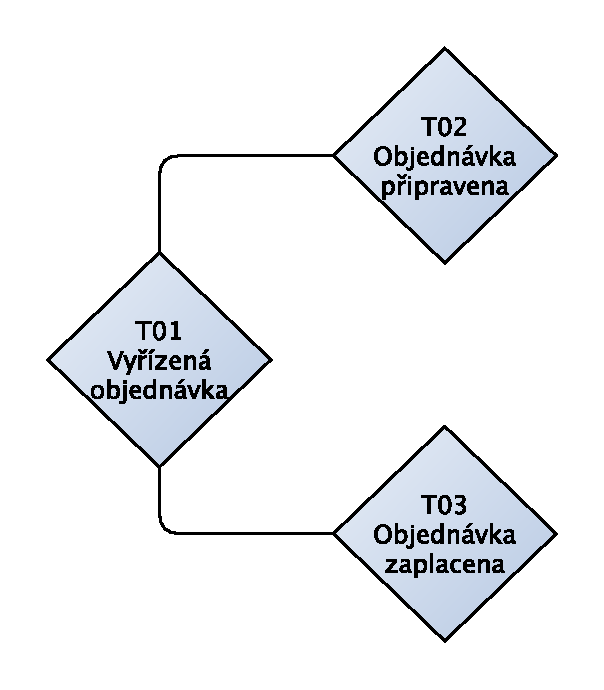
\includegraphics[scale=0.75]{obrazky/result-structure-chart-pizzeria}
\caption{Struktura závislosti transakcí v případu Pizzerie Mama Mia}
\label{fig:result_structure_chart}
\end{figure}

\subsection{Krok 6: Vytvoření DEMO modelů}
V předposledním kroku navržené metody je nutné vytvořit dva DEMO modely. Tyto modely slouží zejména pro zpětnou verifikaci vzniklého BPMN modelu.

Prvním vytvořeným modelem je Actor-Transaction Diagram (ATD), který zachycuje pouze transakce a actory, kteří se transakce účastní. Na obrázku \ref{fig:atd_pizzeria} můžeme vidět ATD pro případ Pizzerie Mama Mia. Zákazníka zde reprezentuje actor CA01 a jako jediný je vně organizace Pizzeria. Dalším actorem je Mia, která v tomto ATD vystupuje pod označením A01 a Mario, který je označen jako A02.

\begin{figure}[H]\centering
\includegraphics[scale=0.35]{obrazky/ATD-pizzeria}
\caption{ATD Pizzerie Mama Mia \cite{Dietz2006}}
\label{fig:atd_pizzeria}
\end{figure}

Pro vytváření výsledného BPMN modelu nám však bude více nápomocný Process Structure Diagram (PSD), který zachycuje všechny transakční kroky dle transakčního vzoru. V kroku 7 bude naším úkolem tyto transakční kroky vyjádřené v PSD popsat pomocí BPMN primitiv, které jsou popsány v sekci \ref{sec:tr_vzor_ulohy_signaly}.

Na \ref{fig:psd_pizzeria} můžem vidět PSD pro případ Pizzerie Mama Mia. Za povšimnutí stojí zejména šipky s přerušovaným tělem, které vyjadřují závislost vykonání C-actu na vykonání C-actu v jiné transakci. Díky tomu lze vidět, že vykonání Request T03 je závislé na Accept T02 a Execution T01 je závislá na Accept T03. Převedeno do lidské řeči to znamená, že než můžeme požádat zákazníka o zaplacení objednávky, musíme jí nejdřív připravit a zákazník ji musí akceptovat a že než je objednávka vyřízena musí dojít k jejímu zaplacení. Toto zjištění nám pomůže při vytváření BPMN modelu určit pořadí aktivit, které budeme propjovat pomocí sekvenčních toků.

\begin{figure}[H]\centering
\includegraphics[scale=0.35]{obrazky/PSD-pizzeria}
\caption{PSD Pizzerie Mama Mia \cite{Dietz2006}}
\label{fig:psd_pizzeria}
\end{figure}

\subsection{Krok 7: Vytvoření BPMN modelu}
Nyní je vše připraveno pro vytvoření konečného BPMN modelu. Při jeho tvorbě budeme vycházet především z PSD modelu vytvořeného v předešlém kroce a z předpisu pro převedení transakčního axiomu do BPMN primitiv, který je uveden v sekci \ref{sec:tr_vzor_ulohy_signaly}. Postupujeme tedy po jednotlivých transakčních krocích zobrazených v PSD v obrázku \ref{fig:psd_pizzeria} a převádíme je dle tohoto předpisu do BPMN. Je důležité správně poskládat aktivity dle závislostí vyjádřených v kroku 5 i v PSD pomocí přerušovaných čar a diskutovaných v předchozím kroku.

Při vytváření PSD v předchozím kroku je použit pouze základní transakční vzor. Důvodem je větší čitelnost výsledného BPMN modelu a také absence popisu nešťastných scénářů v textovém popisu případu Pizzerie Mama Mia. Dle předpisu v sekci \ref{sec:tr_vzor_ulohy_signaly} by však nebyl problém vytvořit i BPMN model ze standardního transakčního vzoru.

Zobrazení případu Pizzerie Mama Mia v BPMN za použití metody navržené v této práci můžeme vidět na obrázku:

\begin{center}
\begin{figure}[H]
\centerline{\includegraphics[width=1.28\textwidth,height=\textheight,keepaspectratio]{obrazky/pizzeria-bpmn-1}}
\caption{Případ Pizzerie Mama Mia v BPMN 1/2}
\label{fig:pizzeria_bpmn_1}
\end{figure}
\end{center}

\begin{center}
\begin{figure}[H]
\centerline{\includegraphics[width=1.28\textwidth,height=\textheight,keepaspectratio]{obrazky/pizzeria-bpmn-2}}
\caption{Případ Pizzerie Mama Mia v BPMN 2/2}
\label{fig:pizzeria_bpmn_2}
\end{figure}
\end{center}

\section{Diskuse}
Na obrázcích \ref{fig:pizzeria_bpmn_1} a \ref{fig:pizzeria_bpmn_2} vidíme, že se nám podařilo vytvořit BPMN model pro případ Pizzerie Mama Mia dle metody navržené v kapitole 5. Vytvořený BPMN model je:

\begin{itemize}
\item \textit{kompletní} dle transakčního axiomu – žádný transakční krok dle základního transakčního vzoru v modelu nechybí a díky použití plaveckých drah je jasné, který actor je zodpovědný za vykonání konkrétního transakčního kroku
\item \textit{konzistentní} dle transakčního axiomu – pořadí provádění všech transakčních kroků je konzistentní se základním transakčním vzorem
\item \textit{jednoznačný} – navržená metoda zajišťuje, že při správném aplikování všech kroků metody vznikne vždy ten samý model
\item \textit{esenciální} – výsledný model neobsahuje žádné implementační detaily. Při jeho tvorbě bylo použito pouze aktivit, které jsme vyhodnotili jako Performa.
\end{itemize}

\subsection{Slabiny metody}
\subsubsection{Modelování komplexních procesů}
Na obrázcích \ref{fig:pizzeria_bpmn_1} a \ref{fig:pizzeria_bpmn_2} jsou zachyceny pouze 3 transakce za použití základního transakčního vzoru a stejně jsme museli diagram rozdělit na 2 obrázky, protože se celý nevešel na jednu stránku. V případě modelování komplexnějších procesů, které obsahují desítky transakcí bude problém jen narůstat a model se bude obtížně vytvářet i číst.

Řešením je v tomto případě automatické generování BPMN diagramu z ATD diagramu (případně PSD dle DEMO 3) , který je mnohem méně obsáhlý a dobře čitelný i když obsahuje desítky transakcí. Pokud by bylo možné automatizovat vytváření BPMN a jejich verifikaci dle DEMO modelů, jednalo by se o velký krok dopředu.

\subsubsection{Korektní provedení kroku 2}
Z mé zkušenosti je pro velké množství lidí velmi problematické správně aplikovat krok 2 navržené metody, neboli správně provést na textovém popisu procesu Performa-Informa-Forma analýzu. Lidská řeč je totiž velmi vágní a rozdíly mezi Performa, Informa i Forma aktivitami jsou často nezřetelné a ani odborníkům se zkušenostmi s DEMO se často nedaří provést tento krok správně.

Na tomto místě je třeba uvést, že i situace, kdy se nepodaří všechny aktivity správně zařadit a jako Performa je napříkad zařazena aktivita, která Performa není, stále pravděpodobně vznikne kvalitnější BPMN model než by vzniknul neaplikováním této metody. Jak popisuje \cite{Silver2011} \uv{špatné BPMN} je dnes spíše pravidlem než výjimkou a aplikace navržené metody by tedy za každých okolností přispěla obecně k lepším výsledkům.

\nocite{*}
\bibliographystyle{plain}
\bibliography{Bibliography}

\end{document}
	
\begin{conclusion}
	Na začátku této práce jsme uvedli důvody, proč je vůbec vhodné se modelování podnikových procesů věnovat – jedná se o cestu k větší efektivitě a udržitelnému růstu každé organizace. K řízení podnikových procesů však existuje celá řada přístupů, které se mění v čase podle toho, jak se mění podniky i technologie. Výkon dnešních výpočetních prostředků je na takové úrovni, že umožňuje  prakticky v reálném čase vyhodnocovat efektivitu provádění podnikového procesu a rychle zavádět úpravy v případě, že se podaří odhalit problém.

Kdo z nás, zákazníků velkých podniků jako jsou banky, telefonní operátoři nebo státní úřady, má pocit, že procesy v těchto organizacích jsou skutečně efektivní, a že při jejich provádění nedochází ke zbytečným prodlevám či plýtvání? Běžně používaným tvrzením v médiích či mezi politiky je to, že jen malé organizace dokáží být efektivní a ty velké jsou naopak „těžkopádné molochy“. Čím je to způsobeno? Ve všech takto velkých organizacích se jistě procesnímu řízení věnují, je tedy možné, že je něco špatně s metodami, podle kterých jsou podnikové procesy v dnešní době řízeny?

Ve druhé kapitole této práce najdeme srovnání nejběžnějších technik pro modelování podnikových procesů, jako jsou vývojové diagramy, UML nebo BPMN a také metodologie DEMO, která je sice v praxi využívána zatím jen málo, její potenciál je ale v mnohém revoluční. Tato metodologie totiž dokáže uvnitř operací různorodých organizací rozpoznat vzory a pomocí nich pak popsat chod celé organizace bez zahlcení detaily, které nejsou podstatné. Tento přístup umožňuje řídícím pracovníkům soustředit se jen na to důležité a přesto získat kompletní informace o vlastním podniku.

Faktem však je, že první verze DEMO vznikly již v 80. letech minulého století a do dnešních dnů se DEMO šíří jen pomalu. O důvodech můžeme jen spekulovat, přesto je dokážeme s určitou mírou jistoty odhadnout. DEMO je totiž poměrně složité na naučení, což stojí podniky čas a úsilí, které zatím nejsou ochotny vynaložit.

Oproti tomu notace BPMN těmito „nedostatky“ netrpí. O popularitě této notace, která vychází z vývojových diagramů, svědčí i fakt, že v dnešní době existuje na trhu několik desítek nástrojů, které ji podporují a nové stále přibývají. BPMN je jednoduchá a přímočará notace, ve které může uživatel začít modelovat „během několika málo hodin“. Důsledkem však je, že vzniká obrovské množství modelů, které svojí kvalitou efektivní řízení procesů v organizaci často spíše komplikují než usnadňují.

Tato práce vznikla na popud Ing. Pavla Náplavy a Stevena Van Kervela z nizozemské firmy Formetis, kteří měli za to, že by kombinací těchto dvou technik mohl vzniknout nadějný nástroj pro zvýšení kvality řízení podnikových procesů. Tato práce se snaží udělat první malý krok tímto směrem v podobě průzkumu možností přenesení základních teoretických konceptů metodologie DEMO do notace BPMN. Zároveň přináší první verzi metody, která na teoretických základech z DEMO umožňuje vytvářet BPMN modely, které nebudou trpět nekompletností či nekonzistentností.

\section{Přínosy práce}
Přínosy této diplomové práce vidí autor ve čtyřech oblastech:

\begin{enumerate}
\item Srovnání nejběžnějších technik pro modelování podnikových procesů z pohledu jejich silných a slabých stránek zejména pro business uživatele
\item Průzkum přínosů spojení DEMO a BPMN
\item Předpis pro vyjádření základních konceptů DEMO pomocí primitiv notace BPMN
\item Návrh první verze metody pro vytváření BPMN modelů podnikových procesů za použití teoretických konceptů z metodologie DEMO
\end{enumerate}

\section{Zjištění}
Z argumentace v kapitolách \ref{chap:2}, \ref{chap:3}, \ref{chap:4} a \ref{chap:5} je zřejmé, že pro spojení obou technik existuje velký prostor, neboť silné stránky jedné techniky doplňují slabé stránky druhé techniky a naopak. Jednoduchost, přímočarost, velké množství dostupných nástrojů a uživatelská základna BPMN na straně jedné a teoretické koncepty, které zajišťují ontologickou kompletnost, konzistentnost, jednoznačnost a esencialitu, na straně DEMO si přímo říkají o nalezení cesty, jak tyto vlastnosti skloubit.

V kapitole \ref{chap:5} je provedena analýza možností, jak skloubení dosáhnout, pomocí diskuse nad možnými přístupy, kterými je možné základní teoretické koncepty DEMO v BPMN vyjádřit. U každého navrženého přístupu je diskutována jednak míra korektnosti s jakou je pomocí takového přístupu možné dosáhnout požadovaných ontologických vlastností a jednak srozumitelnost a přívětivost použití takového přístupu pro business uživatele. 

Podařilo se zjistit, jak dokládá text kapitoly \ref{chap:5}, že je skutečně možné v BPMN vyjádřit požadované koncepty z DEMO s minimální ztrátou korektnosti. BPMN modely, které vznikly aplikací metody navržené v kapitole \ref{chap:5}, jsou skutečně kompletní, konzistentní, jednoznačné a esenciální. Situací, které můžeme modelovat v BPMN, je však nepřeberné množství a vhodnost navržené metody tak musí být v takových situacích ověřena dalším výzkumem a nadále precizována.

Slabiny navržené metody se nacházejí jednak v modelování komplexních procesů, které obsahují větší množství transakcí. Výsledný model se v takovou chvíli stává poměrně nepřehledným, což v praxi komplikuje jeho následnou analýzu. S tímto problémem se však potýká celé BPMN a navržená metoda ho jen zmírňuje. Nezřídka můžeme vidět v organizacích BPMN modely, které jsou rozprostřené přes několik stran formátu A4. Navržená metoda však ve svém šestém kroku počítá s vytvořením DEMO Actor-Transaction Diagramu, který poskytuje pohled na organizaci na nejvyšší úrovni abstrakce. Tento diagram totiž potřebuje pro zobrazení jedné transakce pouze jeden symbol. Částečným řešením tohoto problému by tak mohlo být generování výsledného BPMN modelu přímo z ATD a PSD diagramů.

Další slabinou navržené metody je hned druhý krok, ve kterém je nutné rozlišit, které aktivity vyjádřené v textovém procesu jsou ontologické, infologické nebo datalogické. Jedná se o poměrně obtížný úkol, se kterým mají čas od času problémy i zkušení profesionálové. Řešení v tomto případě neexistuje, tuto dovednost lze získat pouze praxí.

\section{Další výzkum}
Závěry této práce poskytují obrovský prostor pro další výzkum. Vzhledem k tomu, že se jedná o první návrh metody, která kombinuje BPMN a DEMO, je třeba dalším výzkumem prověřit prakticky veškerá východiska, na kterých staví. Zejména pak vhodnost použití konkrétních BPMN primitiv pro vyjádření konceptů metodologie DEMO jako jsou agenda, C-act, C-fact, P-act, P-fact a další.

Velká příležitost pro další výzkum se rovněž skýtá v oblasti automatizace některých částí této metody a v oblasti simulace výsledného BPMN modelu. V tomto případě by bylo vhodné analyzovat možnosti DEMO softwarového enginu, který vyvíjí firma Formetis, a implementovat rozšíření, které by umožnilo jednak z DEMO modelů automaticky generovat BPMN modely s vlastnostmi, které DEMO zajišťuje a dále simulovat běh a agendu BPMN modelu. Veškeré možnosti pro další výzkum jsou popsány v sekci \ref{sec:dalsi_vyzkum}.
\end{conclusion}

\nocite{*}
\bibliographystyle{csn690}
\bibliography{Bibliography}

\appendix

\chapter{Seznam použitých zkratek}
% \printglossaries
\begin{description}
	\item[ABD] Actor Bank Diagram
	\item[AM] Action Model
	\item[ATD] Actor-Transaction Diagram
	\item[BCT] Bank Contents Table
	\item[BPMN] Business Process Model and Notation
	\item[BPEL] Business Process Execution Language
	\item[BPM] Business Process Management
	\item[BPMI] Business Process Management Initiative
	\item[BPML] Business Process Management Language
	\item[BPMS] Business Process Management Software
	\item[CMM] Capability Maturity Model
	\item[DEMO] Design \& Engineering Methodology for Organizations
	\item[IAM] Interaction Model
	\item[ISM] Interstriction Model
	\item[IUT] Information Use Table
	\item[JIT] Just In Time
	\item[OCD] Organization Construction Diagram
	\item[OFD] Object Fact Diagram
	\item[OPL] Object Property List
	\item[OMG] Object Management Group
	\item[PSD] Process Structure Diagram
	\item[SM] State Model
	\item[TQM] Total Quality Management
	\item[TRT] Transaction Result Table
	\item[UML] Unified Modeling Language
	\item[WSDL] Web Services Description Language
\end{description}

\chapter{Glosář}
\begin{description}
	\item[Black Box Model] Jako \uv{Black Box Model} označujeme model systému, u kterého víme, že určitým způsobem přeměňuje vstupy na výstupy, ale nevíme, jak funguje uvnitř.
	\item[White Box Model] Jako \uv{White Box Model} označujeme model systému, u kterého víme, že určitým způsobem přeměňuje vstupy na výstupy, ale také to, jak k tomu dochází. Víme tedy, jak takový systém funguje uvnitř.
	\item[WSDL – Web Service Description Language] Jazyk pro popis webové služby z pohledu poskytovaných funkcionalit a možností, jak je používat z vnějšku.
	\item[XML – Extensible Markup Language] Značkovací jazyk používaný většinou ke specifikaci struktury uvnitř různých typů dat pro účely dalšího zpracování.
\end{description}

% % % % % % % % % % % % % % % % % % % % % % % % % % % % 
% % Tuto kapitolu z výsledné práce ODSTRAŇTE.
% % % % % % % % % % % % % % % % % % % % % % % % % % % % 
% 
% \chapter{Návod k~použití této šablony}
% 
% Tento dokument slouží jako základ pro napsání závěrečné práce na Fakultě informačních technologií ČVUT v~Praze.
% 
% \section{Výběr základu}
% 
% Vyberte si šablonu podle druhu práce (bakalářská, diplomová), jazyka (čeština, angličtina) a kódování (ASCII, \mbox{UTF-8}, \mbox{ISO-8859-2} neboli latin2 a nebo \mbox{Windows-1250}). 
% 
% V~české variantě naleznete šablony v~souborech pojmenovaných ve formátu práce\_kódování.tex. Typ může být:
% \begin{description}
% 	\item[BP] bakalářská práce,
% 	\item[DP] diplomová (magisterská) práce.
% \end{description}
% Kódování, ve kterém chcete psát, může být:
% \begin{description}
% 	\item[UTF-8] kódování Unicode,
% 	\item[ISO-8859-2] latin2,
% 	\item[Windows-1250] znaková sada 1250 Windows.
% \end{description}
% V~případě nejistoty ohledně kódování doporučujeme následující postup:
% \begin{enumerate}
% 	\item Otevřete šablony pro kódování UTF-8 v~editoru prostého textu, který chcete pro psaní práce použít -- pokud můžete texty s~diakritikou normálně přečíst, použijte tuto šablonu.
% 	\item V~opačném případě postupujte dále podle toho, jaký operační systém používáte:
% 	\begin{itemize}
% 		\item v~případě Windows použijte šablonu pro kódování \mbox{Windows-1250},
% 		\item jinak zkuste použít šablonu pro kódování \mbox{ISO-8859-2}.
% 	\end{itemize}
% \end{enumerate}
% 
% 
% V~anglické variantě jsou šablony pojmenované podle typu práce, možnosti jsou:
% \begin{description}
% 	\item[bachelors] bakalářská práce,
% 	\item[masters] diplomová (magisterská) práce.
% \end{description}
% 
% \section{Použití šablony}
% 
% Šablona je určena pro zpracování systémem \LaTeXe{}. Text je možné psát v~textovém editoru jako prostý text, lze však také využít specializovaný editor pro \LaTeX{}, např. Kile.
% 
% Pro získání tisknutelného výstupu z~takto vytvořeného souboru použijte příkaz \verb|pdflatex|, kterému předáte cestu k~souboru jako parametr. Vhodný editor pro \LaTeX{} toto udělá za Vás. \verb|pdfcslatex| ani \verb|cslatex| \emph{nebudou} s~těmito šablonami fungovat.
% 
% Více informací o~použití systému \LaTeX{} najdete např. v~\cite{wikilatex}.
% 
% \subsection{Typografie}
% 
% Při psaní dodržujte typografické konvence zvoleného jazyka. České \uv{uvozovky} zapisujte použitím příkazu \verb|\uv|, kterému v~parametru předáte text, jenž má být v~uvozovkách. Anglické otevírací uvozovky se v~\LaTeX{}u zadávají jako dva zpětné apostrofy, uzavírací uvozovky jako dva apostrofy. Často chybně uváděný symbol "{} (palce) nemá s~uvozovkami nic společného.
% 
% Dále je třeba zabránit zalomení řádky mezi některými slovy, v~češtině např. za jednopísmennými předložkami a spojkami (vyjma \uv{a}). To docílíte vložením pružné nezalomitelné mezery -- znakem \texttt{\textasciitilde}. V~tomto případě to není třeba dělat ručně, lze použít program \verb|vlna|.
% 
% Více o~typografii viz \cite{kobltypo}.
% 
% \subsection{Obrázky}
% 
% Pro umožnění vkládání obrázků je vhodné použít balíček \verb|graphicx|, samotné vložení se provede příkazem \verb|\includegraphics|. Takto je možné vkládat obrázky ve formátu PDF, PNG a JPEG jestliže používáte pdf\LaTeX{} nebo ve formátu EPS jestliže používáte \LaTeX{}. Doporučujeme preferovat vektorové obrázky před rastrovými (vyjma fotografií).
% 
% \subsubsection{Získání vhodného formátu}
% 
% Pro získání vektorových formátů PDF nebo EPS z~jiných lze použít některý z~vektorových grafických editorů. Pro převod rastrového obrázku na vektorový lze použít rasterizaci, kterou mnohé editory zvládají (např. Inkscape). Pro konverze lze použít též nástroje pro dávkové zpracování běžně dodávané s~\LaTeX{}em, např. \verb|epstopdf|.
% 
% \subsubsection{Plovoucí prostředí}
% 
% Příkazem \verb|\includegraphics| lze obrázky vkládat přímo, doporučujeme však použít plovoucí prostředí, konkrétně \verb|figure|. Například obrázek \ref{fig:float} byl vložen tímto způsobem. Vůbec přitom nevadí, když je obrázek umístěn jinde, než bylo původně zamýšleno -- je tomu tak hlavně kvůli dodržení typografických konvencí. Namísto vynucování konkrétní pozice obrázku doporučujeme používat odkazování z~textu (dvojice příkazů \verb|\label| a \verb|\ref|).
% 
% \begin{figure}\centering
% 	\includegraphics[width=0.5\textwidth, angle=30]{cvut-logo-bw}
% 	\caption[Příklad obrázku]{Ukázkový obrázek v~plovoucím prostředí}\label{fig:float}
% \end{figure}
% 
% \subsubsection{Verze obrázků}
% 
% % Gnuplot BW i barevně
% Může se hodit mít více verzí stejného obrázku, např. pro barevný či černobílý tisk a nebo pro prezentaci. S~pomocí některých nástrojů na generování grafiky je to snadné.
% 
% Máte-li například graf vytvořený v programu Gnuplot, můžete jeho černobílou variantu (viz obr. \ref{fig:gnuplot-bw}) vytvořit parametrem \verb|monochrome dashed| příkazu \verb|set term|. Barevnou variantu (viz obr. \ref{fig:gnuplot-col}) vhodnou na prezentace lze vytvořit parametrem \verb|colour solid|.
% 
% \begin{figure}\centering
% 	\includegraphics{gnuplot-bw}
% 	\caption{Černobílá varianta obrázku generovaného programem Gnuplot}\label{fig:gnuplot-bw}
% \end{figure}
% 
% \begin{figure}\centering
% 	\includegraphics{gnuplot-col}
% 	\caption{Barevná varianta obrázku generovaného programem Gnuplot}\label{fig:gnuplot-col}
% \end{figure}
% 
% 
% \subsection{Tabulky}
% 
% Tabulky lze zadávat různě, např. v~prostředí \verb|tabular|, avšak pro jejich vkládání platí to samé, co pro obrázky -- použijte plovoucí prostředí, v~tomto případě \verb|table|. Například tabulka \ref{tab:matematika} byla vložena tímto způsobem.
% 
% \begin{table}\centering
% 	\caption[Příklad tabulky]{Zadávání matematiky}\label{tab:matematika}
% 	\begin{tabular}{|l|l|c|c|}\hline
% 		Typ		& Prostředí		& \LaTeX{}ovská zkratka	& \TeX{}ovská zkratka	\tabularnewline \hline \hline
% 		Text		& \verb|math|		& \verb|\(...\)|	& \verb|$...$|		\tabularnewline \hline
% 		Displayed	& \verb|displaymath|	& \verb|\[...\]|	& \verb|$$...$$|	\tabularnewline \hline
% 	\end{tabular}
% \end{table}
% 
% % % % % % % % % % % % % % % % % % % % % % % % % % % % 

\chapter{Obsah přiloženého CD}

%upravte podle skutecnosti

\begin{figure}
	\dirtree{%
		.1 readme.txt\DTcomment{stručný popis obsahu CD}.
		.1 exe\DTcomment{adresář se spustitelnou formou implementace}.
		.1 src.
		.2 impl\DTcomment{zdrojové kódy implementace}.
		.2 thesis\DTcomment{zdrojová forma práce ve formátu \LaTeX{}}.
		.1 text\DTcomment{text práce}.
		.2 thesis.pdf\DTcomment{text práce ve formátu PDF}.
		.2 thesis.ps\DTcomment{text práce ve formátu PS}.
	}
\end{figure}

\end{document}
